%\documentclass[aps,prb,onecolumn,nofootinbib]{revtex4}  
\documentclass[12pt,a4paper]{article}
\usepackage[margin=1in]{geometry}  % set the margins to 1in on all sides
%\usepackage{jheppub}
\usepackage{amsmath,amsfonts,amssymb,latexsym,dsfont}
\usepackage{hhline}
\usepackage{amsthm}
\newtheorem{theorem}{Theorem}[subsection]
\newtheorem{axiom}[theorem]{Axiom}
\newtheorem{lemma}[theorem]{Lemma}
\usepackage{graphicx}
%\usepackage[arrow,matrix]{xy}
\usepackage[all]{xy}
\usepackage{tikz}
\usepackage{tikz-cd}
\definecolor{hanpurple}{rgb}{0.32, 0.09, 0.98}
\setcounter{MaxMatrixCols}{12}
\usepackage{tabu}

\usepackage[numbers]{natbib}
\usepackage[colorlinks]{hyperref}
\hypersetup{linkcolor={hanpurple}}


\usetikzlibrary{positioning,arrows}
\usetikzlibrary{decorations.pathmorphing}
\usetikzlibrary{decorations.markings}

\usetikzlibrary{decorations.pathreplacing,calc}

\newcommand{\tikzmark}[2][-3pt]{\tikz[remember picture, overlay, baseline=-0.5ex]\node[#1](#2){};}

\tikzset{brace/.style={decorate, decoration={brace}},
 brace mirrored/.style={decorate, decoration={brace,mirror}},
}

\newcounter{brace}
\setcounter{brace}{0}
\newcommand{\drawbrace}[3][brace]{%
 \refstepcounter{brace}
 \tikz[remember picture, overlay]\draw[#1] (#2.center)--(#3.center)node[pos=0.5, name=brace-\thebrace]{};
}

\newcounter{arrow}
\setcounter{arrow}{0}
\newcommand{\drawcurvedarrow}[3][]{%
 \refstepcounter{arrow}
 \tikz[remember picture, overlay]\draw (#2.center)edge[#1]node[coordinate,pos=0.5, name=arrow-\thearrow]{}(#3.center);
}

% #1 options, #2 position, #3 text 
\newcommand{\annote}[3][]{%
 \tikz[remember picture, overlay]\node[#1] at (#2) {#3};
}

\newcommand{\tp}{\otimes}
\newcommand{\tpc}{\tilde{\otimes}}
\newcommand{\ra}{\rightarrow}
\newcommand{\unit}{\mathds{1}}
\newcommand{\zz}{\mathbb{Z}}
\newcommand{\mce}{\mathcal{E}}
\newcommand{\mcb}{\mathcal{B}}
\newcommand{\cc}{\mathbb{C}}
\newcommand{\rr}{\mathbb{R}}
\newcommand{\mcr}{\mathcal{R}}
\newcommand{\mcz}{\mathcal{Z}}
\newcommand{\mca}{\mathcal{A}}
\newcommand{\mcd}{\mathcal{D}}
\newcommand{\mcg}{\mathcal{G}}
\newcommand{\mct}{\mathcal{T}}
\newcommand{\mcs}{\mathcal{S}}
\newcommand{\mch}{\mathcal{H}}
\newcommand{\mcl}{\mathcal{L}}
\newcommand{\mcc}{\mathcal{C}}
\newcommand{\mck}{\mathcal{K}}
\newcommand{\mco}{\mathcal{O}}
\newcommand{\mcm}{\mathcal{M}}
\newcommand{\mcp}{\mathcal{P}}
\newcommand{\mcv}{\mathcal{V}}
\newcommand{\mcx}{\mathcal{X}}
\newcommand{\ul}{\underline}
\newcommand{\Mod}{\text{Mod}}
\newcommand{\Aut}{\text{Aut}}
\newcommand{\ulmcc}{\underline{\mathcal{C}}}
\newcommand{\zt}{\mathbb{Z}_2}
\newcommand{\oeo}{\text{others = 1}}
\newcommand\be            {\begin{equation}}
\newcommand\ee            {\end{equation}}
\newcommand\ba            {\begin{aligned}}
\newcommand\ea            {\end{aligned}}
\newcommand{\mcf}{\mathcal{F}}
\newcommand{\spinz}{\text{\sffamily{Z}}}
\newcommand{\spinx}{\text{\sffamily{X}}}
\newcommand{\zc}{\mathcal{Z}(\mathcal{C})}
\newcommand{\id}{\text{id}}
\newcommand{\Hom}{\text{Hom}}
\newcommand{\mor}{\text{mor}}
\newcommand{\obj}{\text{obj}}
\newcommand{\End}{\text{End}}
\newcommand{\Tor}{\text{Tor}}
\newcommand{\Ext}{\text{Ext}}
\newcommand{\p}{\partial}
\newcommand{\wt}{\widetilde}
\usepackage{verbatim}
\newcommand{\cl}{\mathbb{C}\ell}
\newcommand{\vect}{\text{Vec}}
\newcommand{\svect}{\text{sVec}}
\newcommand{\spin}{\text{Spin}}
\newcommand{\pin}{\text{Pin}}
\newcommand{\fube}{\textbf{Tube}}
\newcommand{\tube}{\textbf{Tube}}
\newcommand{\fld}{\mathcal{F}} %fld was for field config
\newcommand{\Tr}{\text{Tr}}

%%
\newcommand{\sob}{\text{sob}_r}
%\sob(\mcc) = list of representatives of isomorphism classes of simple objects
\newcommand{\sobi}{\text{sob}_i} 
%\sobi(\mcc) = list of simple objects of \mcc.

% KW
\newcommand{\ot}{\otimes}
\newcommand{\bd}{\partial}
\DeclareMathOperator{\Arf}{Arf}
\definecolor{kwcolor}{rgb}{0.2, 0.5, 0.85}
\newcommand{\kw}[1]{{\color{kwcolor}\footnotesize{(KW) #1}}}
\newcommand{\kwsep}{\bigskip\hrule\medskip\hrule\medskip\hrule\bigskip}
% \nn is for compatibility with stuff copied from my other papers; can be deleted eventually
\newcommand{\nn}[1]{{\color{kwcolor}[#1]}}

\newcommand{\bra}[1]{\ensuremath{\left\langle#1\right|}}
\newcommand{\ket}[1]{\ensuremath{\left|#1\right\rangle}}

\definecolor{ao(english)}{rgb}{0.0, 0.5, 0.0}
\definecolor{americanrose}{rgb}{1.0, 0.01, 0.24}
\definecolor{amber(sae/ece)}{rgb}{1.0, 0.49, 0.0}

\newcommand{\dave}[1]{{\color{ao(english)}\footnotesize{(DA) #1}}}
\newcommand{\questionable}[1]{{\color{amber(sae/ece)}\footnotesize{(??) #1}}} %use this to flag questionable stuff

%a purple that looks different from red. EL: nice! I like the name
\definecolor{amethyst}{rgb}{0.6, 0.4, 0.8}
\newcommand{\ethan}[1]{{\color{amethyst}\footnotesize{(EL) #1}}}

\newcommand{\abullet}{{\color{amethyst} \bullet}}


\newcommand{\CapDotLeft}{\mathord{\vcenter{\hbox{
\includegraphics[scale=1]{CapDotLeft.pdf}}}}}
\newcommand{\CapDotRight}{\mathord{\vcenter{\hbox{
\includegraphics[scale=1]{CapDotRight.pdf}}}}}
\newcommand{\CupDotLeft}{\mathord{\vcenter{\hbox{
\includegraphics[scale=1,angle=180,origin=c]{CapDotRight.pdf}}}}}
\newcommand{\CupDotRight}{\mathord{\vcenter{\hbox{
\includegraphics[scale=1,angle=180,origin=c]{CapDotLeft.pdf}}}}}



\newcommand{\CupCapPsi}{\mathord{\vcenter{\hbox{
\includegraphics[scale=1]{cupcappsi.pdf}}}}}

\newcommand{\Qcap}{\mathord{\vcenter{\hbox{
\includegraphics[scale=1]{Qcap.pdf}}}}}
\newcommand{\Qcup}{\mathord{\vcenter{\hbox{
\includegraphics[scale=1,angle=180,origin=c]{Qcap.pdf}}}}}
\newcommand{\Qdotdot}{\mathord{\vcenter{\hbox{\includegraphics[scale=1]{Qdotdot.pdf}}}}}
\newcommand{\QIdentity}{\mathord{\vcenter{\hbox{
\includegraphics[scale=1]{QIdentity.pdf}}}}}

\newcommand{\CupCap}{\mathord{\vcenter{\hbox{
\includegraphics[scale=1]{CupCap.pdf}}}}}
\newcommand{\CupCapDots}{\mathord{\vcenter{\hbox{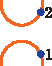
\includegraphics[scale=1]{CupCapDots.pdf}}}}}

\newcommand{\dbeta}{\mathord{\vcenter{\hbox{
\includegraphics[scale=1]{dbeta.pdf}}}}}
\newcommand{\dpsi}{\mathord{\vcenter{\hbox{
\includegraphics[scale=1]{dpsi.pdf}}}}}
\newcommand{\dblank}{\mathord{\vcenter{\hbox{
\includegraphics[scale=1]{dblank.pdf}}}}}





\newcommand{\SigmaDotDot}{\mathord{\vcenter{\hbox{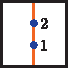
\includegraphics[scale=1]{SigmaDotDot.pdf}}}}}
\newcommand{\SigmaDotDotExchange}{\mathord{\vcenter{\hbox{
\includegraphics[scale=1]{SigmaDotDotExchange.pdf}}}}}
\newcommand{\TwoLine}{\mathord{\vcenter{\hbox{
\includegraphics[scale=1]{TwoLine.pdf}}}}}
\newcommand{\TwoLineDots}{\mathord{\vcenter{\hbox{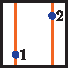
\includegraphics[scale=1]{TwoLineDots.pdf}}}}}


\newcommand{\RDotTwo}{\mathord{\vcenter{\hbox{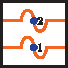
\includegraphics[scale=1]{RDotTwo.pdf}}}}}
\newcommand{\RDotTwoa}{\mathord{\vcenter{\hbox{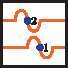
\includegraphics[scale=1]{RDotTwoa.pdf}}}}}
\newcommand{\RDotTwob}{\mathord{\vcenter{\hbox{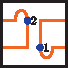
\includegraphics[scale=1]{RDotTwob.pdf}}}}}
\newcommand{\RDotTwoc}{\mathord{\vcenter{\hbox{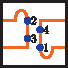
\includegraphics[scale=1]{RDotTwoc.pdf}}}}}

\newcommand{\FubeXXX}{\mathord{\vcenter{\hbox{
\includegraphics[scale=1]{EmptyTube.pdf}}}}}
\newcommand{\FubeXss}{\mathord{\vcenter{\hbox{
\includegraphics[scale=1]{OneLine.pdf}}}}}
\newcommand{\FubeXsds}{\mathord{\vcenter{\hbox{
\includegraphics[scale=1]{OneLineDot.pdf}}}}}



\newcommand{\AnnulusCut}{\mathord{\vcenter{\hbox{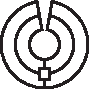
\includegraphics[scale=1]{AnnulusCut.pdf}}}}}
\newcommand{\AnnulusFlat}{\mathord{\vcenter{\hbox{
\includegraphics[scale=1]{AnnulusFlat.pdf}}}}}
\newcommand{\Disc}{\mathord{\vcenter{\hbox{
\includegraphics[scale=1]{Disc.pdf}}}}}
\newcommand{\RotatedTube}{\mathord{\vcenter{\hbox{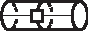
\includegraphics[scale=1]{RotatedTube.pdf}}}}}
\newcommand{\AnnulusGeneric}{\mathord{\vcenter{\hbox{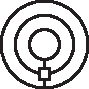
\includegraphics[scale=1]{AnnulusGeneric.pdf}}}}}



\newcommand{\FubeXXXA}{\mathord{\vcenter{\hbox{
\includegraphics[scale=1]{EmptyTubeA.pdf}}}}}
\newcommand{\FubeXssA}{\mathord{\vcenter{\hbox{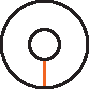
\includegraphics[scale=1]{OneLineA.pdf}}}}}
\newcommand{\FubeXsdsA}{\mathord{\vcenter{\hbox{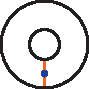
\includegraphics[scale=1]{OneLineDotA.pdf}}}}}

\newcommand{\FubesddXsA}{\mathord{\vcenter{\hbox{
\includegraphics[scale=1]{FubesddXsA.pdf}}}}}

\newcommand{\RDotTwobA}{\mathord{\vcenter{\hbox{
\includegraphics[scale=1]{RDotTwobA.pdf}}}}}\newcommand{\RDotTwocA}{\mathord{\vcenter{\hbox{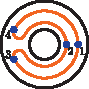
\includegraphics[scale=1]{RDotTwocA.pdf}}}}}


 
\newcommand{\Fubex}[2]{{\mathord{\ooalign{ \vphantom{$\Big|^2$}\cr\hidewidth\ensuremath{\scriptstyle{#2}}\hidewidth\cr$\vcenter{\hbox{$#1$}}$\cr
  \hidewidth\raise0ex\hbox{$\scale{1.2}{\VerticalSpace}$}\cr
  }}}}	




\newcommand{\TubeBC}{\mathord{\vcenter{\hbox{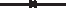
\includegraphics[scale=1]{TubeBC.pdf}}}}}

\newcommand{\TubeBCx}[1]{{\mathord{\ooalign{ \vphantom{$\Big|^2$}\cr\hidewidth\ensuremath{\scriptstyle{#1}}\hidewidth\cr$\vcenter{\hbox{$\scale{1}{\TubeBC}$}}$\cr
  \hidewidth\raise0ex\hbox{$\scale{.25}{\VerticalSpace}$}\cr
  }}}}	

\newcommand{\AnnulusBare}{\mathord{\vcenter{\hbox{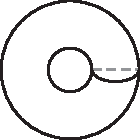
\includegraphics[scale=.6]{AnnulusBare.pdf}}}}}
\newcommand{\AnnularTube}{\mathord{\vcenter{\hbox{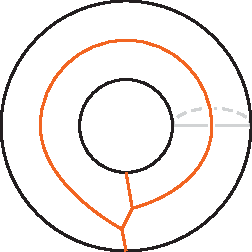
\includegraphics[scale=1]{AnnularTube.pdf}}}}}
\newcommand{\AnnularTubeNoIndex}{\mathord{\vcenter{\hbox{
\includegraphics[scale=1]{AnnularTubeNoIndex.pdf}}}}}
\newcommand{\AnnulusTubeTube}{\mathord{\vcenter{\hbox{
\includegraphics[scale=1]{AnnulusTubeTube.pdf}}}}}

\newcommand{\SAnnulusNoLabel}{\mathord{\vcenter{\hbox{
\includegraphics[scale=1]{SAnnulusNoLabel.pdf}}}}}
\newcommand{\TAnnulusNoLabel}{\mathord{\vcenter{\hbox{\includegraphics[scale=1]{TAnnulusNoLabel.pdf}}}}}


\newcommand{\EdgeTensor}{\mathord{\vcenter{\hbox{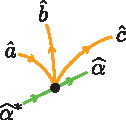
\includegraphics[scale=1]{EdgeTensor.pdf}}}}}

\newcommand{\OneHandleTheta}{\mathord{\vcenter{\hbox{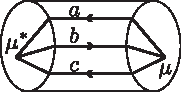
\includegraphics[scale=.7]{OneHandleTheta.pdf}}}}}
\newcommand{\OneHandlemud}{\mathord{\vcenter{\hbox{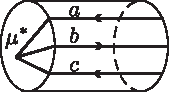
\includegraphics[scale=.7]{OneHandlemud.pdf}}}}}
\newcommand{\OneHandlemu}{\mathord{\vcenter{\hbox{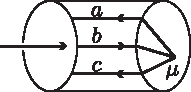
\includegraphics[scale=.7]{OneHandlemu.pdf}}}}}
\newcommand{\OneHandlea}{\mathord{\vcenter{\hbox{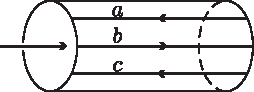
\includegraphics[scale=.7]{OneHandlea.pdf}}}}}

\newcommand{\Tetrahedron}{\mathord{\vcenter{\hbox{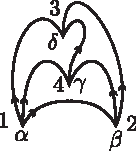
\includegraphics[scale=1]{Tetrahedron.pdf}}}}}
\newcommand{\PitchforkIdempotent}{\mathord{\vcenter{\hbox{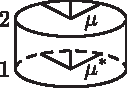
\includegraphics[scale=0.7]{PitchforkIdempotent.pdf}}}}}

\newcommand{\Pitchforkabc}{\mathord{\vcenter{\hbox{\includegraphics[scale=1]{Pitchforkabc.pdf}}}}}
\newcommand{\Pitchforkabcrot}{\mathord{\vcenter{\hbox{\includegraphics[scale=1]{Pitchforkabcrot.pdf}}}}}






\newcommand{\AnnulsLabel}[5]{\mathord{ 
\mkern2mu\overset{#3}{{\Annulusxprime{#1}{#2}}}\mkern2mu\raisebox{0ex}{$\scriptstyle{#4}$} }}

\newcommand*{\Annulus}[2]{{ #1 }
\kern-3.5em\raisebox{1ex}{ $\scriptstyle{#2}$} \kern2.6em} %Could change 0 to 1.2 to raise the B.

\newcommand*{\AnnulusP}[3]{{{\Annulus{#1}{#2}} }
\kern-.5em\raisebox{3.5ex}{ $\scriptstyle{#3}$} \kern.3em} %Could change 0 to 1.2 to raise the B.

\newcommand*{\AnnulusPx}[4]{\AnnulusP{#1}{#2}{#3}
\kern-3.6em\raisebox{-4.5ex}{ $\scriptstyle{#4}$} \kern2.6em} %Could change 0 to 1.2 to raise the B.

\newcommand*{\AnularTubex}[6]{\AnnulusPx{#1}{#2}{#3}{#4}
\kern-4em\raisebox{-4.5ex}{ $\overset{#6}{\underset{#5}{\vphantom{\Big|^2}}}$} \kern3em} %Could change 0 to 1.2 to raise the B.

\newcommand*{\TorusTubex}[6]{\AnnulusPx{#1}{#2}{#3}{#4}
\kern-4em\raisebox{-4.5ex}{ $\overset{#6}{\underset{#5}{\vphantom{\Big|^2}}}$} \kern3em} %Could change 0 to 1.2 to raise the B.

%\newcommand*{\AnnularTubex}[5]{\AnnulusPx{#1}{#2}{}{\; \; \;#3}
%\kern-3.9em\raisebox{-4.5ex}{ $\overset{#5}{\underset{#4}{\vphantom{\Big|^2}}}$} \kern2.7em} %Could change 0 to 1.2 to raise the B.



\newcommand{\SAnnulusx}[3]{\mathrel{\ooalign{$\SAnnulusNoLabel$\cr
  \hidewidth\raise5ex\hbox{$\scriptstyle{#3}\mkern1mu$}\cr
  \hidewidth\raise.8ex\hbox{$\scriptstyle{#2}\mkern63mu$}\cr
    \hidewidth\raise-3.8ex\hbox{$\scriptstyle{#1}\mkern39mu$}\cr
  }}}
  
  \newcommand{\TAnnulusx}[3]{\mathrel{\ooalign{$\TAnnulusNoLabel$\cr
  \hidewidth\raise5ex\hbox{$\scriptstyle{#3}\mkern1mu$}\cr
  \hidewidth\raise.8ex\hbox{$\scriptstyle{#2}\mkern63mu$}\cr
    \hidewidth\raise-4.9ex\hbox{$\scriptstyle{#1}\mkern51mu$}\cr
  }}}

\newcommand{\AnnularTubex}[6]{\mathrel{\ooalign{$#1$\cr
  \hidewidth\raise5ex\hbox{$\scriptstyle{#6}\mkern1mu$}\cr
  \hidewidth\raise.8ex\hbox{$\scriptstyle{#5}\mkern63mu$}\cr
  \hidewidth\raise-.9ex\hbox{$\scriptstyle{#3}\mkern68mu$}\cr
    \hidewidth\raise-4.5ex\hbox{$\scriptstyle{#4} \mkern50mu$}\cr
  \hidewidth\raise-7ex\hbox{$\scriptstyle{#2}\mkern68mu$}\cr
  }}}
  
%\newcommand{\AnnularTubexp}[9]{\mathrel{\ooalign{$#1$\cr
  %\hidewidth\raise5ex\hbox{$\scriptstyle{#9}\mkern1mu$}\cr
 %\hidewidth\raise.8ex\hbox{$\scriptstyle{#8}\mkern63mu$}\cr
 % \hidewidth\raise-3.4ex\hbox{$\scriptstyle{#7}\mkern68mu$}\cr
  %  \hidewidth\raise-5.1ex\hbox{$\scriptstyle{#6}\mkern80mu$}\cr
%  \hidewidth\raise-2.2ex\hbox{$\scriptstyle{#5}\mkern90mu$}\cr
 % \hidewidth\raise-.9ex\hbox{$\scriptstyle{#4}\mkern68mu$}\cr
%    \hidewidth\raise-4.5ex\hbox{$\scriptstyle{#3} \mkern50mu$}\cr
 % \hidewidth\raise-7ex\hbox{$\scriptstyle{#2}\mkern68mu$}\cr
 % }}}



\newcommand{\AnnularTubexp}[9]{\mathrel{\ooalign{$#1$\cr
  \hidewidth\raise5ex\hbox{$\scriptstyle{#9}\mkern1mu$}\cr
 \hidewidth\raise.8ex\hbox{$\scriptstyle{#8}\mkern63mu$}\cr
  \hidewidth\raise-3.7ex\hbox{$\scriptstyle{#7}\mkern50mu$}\cr
    \hidewidth\raise-5.1ex\hbox{$\scriptstyle{#6}\mkern57mu$}\cr
  \hidewidth\raise-2.2ex\hbox{$\scriptstyle{#5}\mkern90mu$}\cr
  \hidewidth\raise-.9ex\hbox{$\scriptstyle{#4}\mkern68mu$}\cr
    \hidewidth\raise-3.8ex\hbox{$\scriptstyle{#3} \mkern69mu$}\cr
  \hidewidth\raise-7ex\hbox{$\scriptstyle{#2}\mkern68mu$}\cr
  }}}


\newcommand{\SmallTorus}[3]{\mathrel{\ooalign{$#1$\cr
  \hidewidth\raise0ex\hbox{$\scriptstyle{#2}\mkern36mu$}\cr
    \hidewidth\raise-1.5ex\hbox{$\scriptstyle{#3}\mkern10mu$}\cr
  }}}
  
  
  \newcommand{\AnnulusTubeTubex}[6]{\mathrel{\ooalign{$#1$\cr
%  \hidewidth\raise5ex\hbox{$\scriptstyle{#7}\mkern1mu$}\cr
  \hidewidth\raise.8ex\hbox{$\scriptstyle{#6}\mkern65mu$}\cr
  \hidewidth\raise-.5ex\hbox{$\scriptstyle{#3}\mkern68mu$}\cr
    \hidewidth\raise-4.9ex\hbox{$\scriptstyle{#4} \mkern50mu$}\cr
     \hidewidth\raise-2.7ex\hbox{$\scriptstyle{#5} \mkern54mu$}\cr
  \hidewidth\raise-7.3ex\hbox{$\scriptstyle{#2}\mkern68mu$}\cr
  }}}
  

  \newcommand{\Cellup}{\mathord{\vcenter{\hbox{\includegraphics[scale=1]{Cellup.pdf}}}}}
    \newcommand{\Celldown}{\mathord{\vcenter{\hbox{\includegraphics[scale=1]{Celldown.pdf}}}}}
        \newcommand{\Cellmid}{\mathord{\vcenter{\hbox{\includegraphics[scale=1]{Cellmid.pdf}}}}}
        \newcommand{\TwoCell}{\mathord{\vcenter{\hbox{\includegraphics[scale=1]{TwoCell.pdf}}}}}
                \newcommand{\Onecell}{\mathord{\vcenter{\hbox{\includegraphics[scale=1]{Onecell.pdf}}}}}      
        
        

 


\newcommand{\TorusLocalRelationc}{\mathord{\vcenter{\hbox{\includegraphics[scale=1]{TorusLocalRelationc.pdf}}}}}
\newcommand{\TorusLocalRelationb}{\mathord{\vcenter{\hbox{\includegraphics[scale=1]{TorusLocalRelationb.pdf}}}}}
\newcommand{\TorusLocalRelationa}{\mathord{\vcenter{\hbox{\includegraphics[scale=1]{TorusLocalRelationa.pdf}}}}}


\newcommand{\Dv}{\mathord{\vcenter{\hbox{\includegraphics[scale=1]{Dv.pdf}}}}}
\newcommand{\Dfv}{\mathord{\vcenter{\hbox{\includegraphics[scale=1]{Dfv.pdf}}}}}


\newcommand{\Horseshoe}{\mathord{\vcenter{\hbox{\includegraphics[scale=1]{Horseshoe.pdf}}}}}
\newcommand{\HorseshoeTwist}{\mathord{\vcenter{\hbox{\includegraphics[scale=1]{HorseshoeTwist.pdf}}}}}
\newcommand{\euv}{\mathord{\vcenter{\hbox{\includegraphics[scale=1]{euv.pdf}}}}}
\newcommand{\chieuv}{\mathord{\vcenter{\hbox{\includegraphics[scale=1]{chieuv.pdf}}}}}


\newcommand{\TubeElement}{\mathord{\vcenter{\hbox{\includegraphics[scale=1]{TubeElement.pdf}}}}}


\newcommand{\LoopOverId}{\mathord{\vcenter{\hbox{\includegraphics[scale=1]{LoopOverId.pdf}}}}}
\newcommand{\Ida}{\mathord{\vcenter{\hbox{\includegraphics[scale=1]{Ida.pdf}}}}}
\newcommand{\OmegaSLoop}{\mathord{\vcenter{\hbox{\includegraphics[scale=1]{OmegaSLoop.pdf}}}}}

\newcommand{\IdxOmegaLoopa}{\mathord{\vcenter{\hbox{\includegraphics[scale=1]{IdxOmegaLoopa.pdf}}}}}
\newcommand{\IdxOmegaLoopb}{\mathord{\vcenter{\hbox{\includegraphics[scale=1]{IdxOmegaLoopb.pdf}}}}}


\newcommand{\HandleSlidea}{\mathord{\vcenter{\hbox{\includegraphics[scale=1]{HandleSlidea.pdf}}}}}
\newcommand{\HandleSlideb}{\mathord{\vcenter{\hbox{\includegraphics[scale=1]{HandleSlideb.pdf}}}}}


\newcommand{\TubeBasisa}{\mathord{\vcenter{\hbox{\includegraphics[scale=1]{TubeBasisa.pdf}}}}}
\newcommand{\TubeBasisb}{\mathord{\vcenter{\hbox{\includegraphics[scale=1]{TubeBasisb.pdf}}}}}
\newcommand{\TubeBasisc}{\mathord{\vcenter{\hbox{\includegraphics[scale=1]{TubeBasisc.pdf}}}}}
\newcommand{\TubeBasisd}{\mathord{\vcenter{\hbox{\includegraphics[scale=1]{TubeBasisd.pdf}}}}}
\newcommand{\TubeBasisdprime}{\mathord{\vcenter{\hbox{\includegraphics[scale=1]{TubeBasisdprime.pdf}}}}}


\newcommand{\gxyaj}{\mathord{\vcenter{\hbox{\includegraphics[scale=1]{gxyaj.pdf}}}}}
\newcommand{\hxyai}{\mathord{\vcenter{\hbox{\includegraphics[scale=1]{hxyai.pdf}}}}}

\newcommand{\VxyaoVxya}{\mathord{\vcenter{\hbox{\includegraphics[scale=1]{VxyaoVxya.pdf}}}}}
\newcommand{\idaprime}{\mathord{\vcenter{\hbox{\includegraphics[scale=1]{idaprime.pdf}}}}}

\newcommand{\Vxyxy}{\mathord{\vcenter{\hbox{\includegraphics[scale=1]{Vxyxy.pdf}}}}}
\newcommand{\idxy}{\mathord{\vcenter{\hbox{\includegraphics[scale=1]{idxy.pdf}}}}}
\newcommand{\Vxyxyomega}{\mathord{\vcenter{\hbox{\includegraphics[scale=1]{Vxyxyomega.pdf}}}}}



\newcommand{\SpinStructureProjector}{\mathord{\vcenter{\hbox{\includegraphics[scale=1]{SpinStructureProjector.pdf}}}}}


\newcommand{\EmptyTubeW}{\mathord{\vcenter{\hbox{\includegraphics[scale=1]{EmptyTubeW.pdf}}}}}

\newcommand{\TubeProject}{\mathord{\vcenter{\hbox{\includegraphics[scale=1]{TubeProject.pdf}}}}}


\newcommand{\TuberraJ}{\mathord{\vcenter{\hbox{\includegraphics[scale=1]{TuberraJ.pdf}}}}}
\newcommand{\Tubeidr}{\mathord{\vcenter{\hbox{\includegraphics[scale=1]{Tubeidr.pdf}}}}}
\newcommand{\Tuberr}{\mathord{\vcenter{\hbox{\includegraphics[scale=1]{Tuberr.pdf}}}}}


\newcommand{\TuberrTraceCe}{\mathord{\vcenter{\hbox{\includegraphics[scale=1]{TuberrTraceCe.pdf}}}}}
\newcommand{\TuberrTraceCo}{\mathord{\vcenter{\hbox{\includegraphics[scale=1]{TuberrTraceCo.pdf}}}}}



\newcommand{\exyomegaa}{\mathord{\vcenter{\hbox{\includegraphics[scale=1]{exyomegaa.pdf}}}}}
\newcommand{\exyomegab}{\mathord{\vcenter{\hbox{\includegraphics[scale=1]{exyomegab.pdf}}}}}
\newcommand{\exyomegac}{\mathord{\vcenter{\hbox{\includegraphics[scale=1]{exyomegac.pdf}}}}}

\newcommand{\EFunctora}{\mathord{\vcenter{\hbox{\includegraphics[scale=1]{EFunctora.pdf}}}}}
\newcommand{\EFunctorb}{\mathord{\vcenter{\hbox{\includegraphics[scale=1]{EFunctorb.pdf}}}}}
\newcommand{\EFunctorc}{\mathord{\vcenter{\hbox{\includegraphics[scale=1]{EFunctorc.pdf}}}}}



\newcommand{\TubeIdempotentTwoStrand}{\mathord{\vcenter{\hbox{\includegraphics[scale=1]{TubeIdempotentTwoStrand.pdf}}}}}
\newcommand{\fTubeCf}{\mathord{\vcenter{\hbox{\includegraphics[scale=1]{fTubeCf.pdf}}}}}
\newcommand{\fTubefOdd}{\mathord{\vcenter{\hbox{\includegraphics[scale=1]{fTubefOdd.pdf}}}}}
\newcommand{\minimalBosonic}{\mathord{\vcenter{\hbox{\includegraphics[scale=1]{minimalBosonic.pdf}}}}}



\newcommand{\FusionIsomorphism}{\mathord{\vcenter{\hbox{\includegraphics[scale=1]{FusionIsomorphism.pdf}}}}}


\newcommand{\TubeCompletea}{\mathord{\vcenter{\hbox{\includegraphics[scale=1]{TubeCompletea.pdf}}}}}
\newcommand{\TubeCompleteb}{\mathord{\vcenter{\hbox{\includegraphics[scale=1]{TubeCompleteb.pdf}}}}}
\newcommand{\TubeCompletec}{\mathord{\vcenter{\hbox{\includegraphics[scale=1]{TubeCompletec.pdf}}}}}
\newcommand{\TubeCompletecprime}{\mathord{\vcenter{\hbox{\includegraphics[scale=1]{TubeCompletecprime.pdf}}}}}



\newcommand{\Ufghk}{\mathord{\vcenter{\hbox{\includegraphics[scale=1]{Ufghk.pdf}}}}}


\newcommand{\fxyaJ}{\mathord{\vcenter{\hbox{\includegraphics[scale=1]{fxyaJ.pdf}}}}}


\newcommand{\TubeTwotoOneStrand}{\mathord{\vcenter{\hbox{\includegraphics[scale=1]{TubeTwotoOneStrand.pdf}}}}}
\newcommand{\TubeOnetoTwoStrand}{\mathord{\vcenter{\hbox{\includegraphics[scale=1]{TubeOnetoTwoStrand.pdf}}}}}
 

\newcommand{\SMatrix}[2]{\mathrel{\ooalign{$\OmegaSLoop$\cr
  \hidewidth\raise0ex\hbox{$\scriptstyle{#1}\mkern18mu$}\cr
    \hidewidth\raise0ex\hbox{$\scriptstyle{#2}\mkern-10mu$}\cr
  }}}
  
  
  \newcommand{\SMatrixx}[2]{\mathrel{\ooalign{$\OmegaSLoop$\cr
  \hidewidth\raise0ex\hbox{$\scriptstyle{#1}\mkern12mu$}\cr
    \hidewidth\raise0ex\hbox{$\scriptstyle{#2}\mkern-10mu$}\cr
  }}}
  
  \newcommand{\OmegaLoopDefectx}[2]{\mathrel{\ooalign{$\OmegaLoopDefect$\cr
  \hidewidth\raise0ex\hbox{$\scriptstyle{#1}\mkern8mu$}\cr
    \hidewidth\raise0ex\hbox{$\scriptstyle{#2}\mkern-22mu$}\cr
  }}}
  
  \newcommand{\OmegaLoopDefect}{\mathord{\vcenter{\hbox{\includegraphics[scale=1]{OmegaLoopDefect.pdf}}}}}
    \newcommand{\DiscGray}{\mathord{\vcenter{\hbox{\includegraphics[scale=1]{DiscGray.pdf}}}}}
    
    
    
\newcommand{\DCSmatrixf}{\mathord{\vcenter{\hbox{\includegraphics[scale=1]{DCSmatrixf.pdf}}}}}
\newcommand{\DCSmatrixa}{\mathord{\vcenter{\hbox{\includegraphics[scale=1]{DCSmatrixa.pdf}}}}}
\newcommand{\DCSmatrixb}{\mathord{\vcenter{\hbox{\includegraphics[scale=1]{DCSmatrixb.pdf}}}}}\newcommand{\DCSmatrixc}{\mathord{\vcenter{\hbox{\includegraphics[scale=1]{DCSmatrixc.pdf}}}}}
\newcommand{\DCSmatrixd}{\mathord{\vcenter{\hbox{\includegraphics[scale=1]{DCSmatrixd.pdf}}}}}
\newcommand{\DCSmatrixe}{\mathord{\vcenter{\hbox{\includegraphics[scale=1]{DCSmatrixe.pdf}}}}}

\newcommand{\DCSmatrixg}{\mathord{\vcenter{\hbox{\includegraphics[scale=1]{DCSmatrixg.pdf}}}}}
\newcommand{\DCSmatrixh}{\mathord{\vcenter{\hbox{\includegraphics[scale=1]{DCSmatrixh.pdf}}}}}


\newcommand{\STorusBasisa}{\mathord{\vcenter{\hbox{\includegraphics[scale=1]{STorusBasisa.pdf}}}}}


\newcommand{\Scalcae}{\mathord{\vcenter{\hbox{\includegraphics[scale=1]{Scalcae.pdf}}}}}  
\newcommand{\Scalcad}{\mathord{\vcenter{\hbox{\includegraphics[scale=1]{Scalcad.pdf}}}}}  
\newcommand{\Scalcac}{\mathord{\vcenter{\hbox{\includegraphics[scale=1]{Scalcac.pdf}}}}}  
\newcommand{\Scalcab}{\mathord{\vcenter{\hbox{\includegraphics[scale=1]{Scalcab.pdf}}}}}
\newcommand{\Scalcaa}{\mathord{\vcenter{\hbox{\includegraphics[scale=1]{Scalcaa.pdf}}}}}  


\newcommand{\Scalcbe}{\mathord{\vcenter{\hbox{\includegraphics[scale=1]{Scalcbe.pdf}}}}}  
\newcommand{\Scalcbd}{\mathord{\vcenter{\hbox{\includegraphics[scale=1]{Scalcbd.pdf}}}}}  
\newcommand{\Scalcbc}{\mathord{\vcenter{\hbox{\includegraphics[scale=1]{Scalcbc.pdf}}}}}  
\newcommand{\Scalcbb}{\mathord{\vcenter{\hbox{\includegraphics[scale=1]{Scalcbb.pdf}}}}}
\newcommand{\Scalcba}{\mathord{\vcenter{\hbox{\includegraphics[scale=1]{Scalcba.pdf}}}}}  


\newcommand{\Scalcbedot}{\mathord{\vcenter{\hbox{\includegraphics[scale=1]{Scalcbedot.pdf}}}}}  
\newcommand{\Scalcbddot}{\mathord{\vcenter{\hbox{\includegraphics[scale=1]{Scalcbddot.pdf}}}}}  
\newcommand{\Scalcbadot}{\mathord{\vcenter{\hbox{\includegraphics[scale=1]{Scalcbadot.pdf}}}}}    
  

  
%\newcommand{\SMatrix}[2]{\mathrel{\ooalign{$\OmegaSLoop$
%\mathrel{\raisebox{#1}{$\oldsqsubset$}}
  %\hidewidth\raise0ex\hbox{$\scriptstyle{a}\mkern0mu$}\cr
    %\hidewidth\raise0ex\hbox{$\scriptstyle{b}\mkern0mu$}\cr
%    \hidewidth\raise-4.3ex\hbox{$\scriptstyle{#2}\mkern43mu$}\cr
%        \hidewidth\raise-6.3ex\hbox{$\scriptstyle{#2}\mkern61mu$}\cr
%        \hidewidth\raise4.1ex\hbox{$\scriptstyle{#4}\mkern25mu$}\cr
  %              \hidewidth\raise-0.3ex\hbox{$\scriptstyle{#3}\mkern60mu$}\cr
%          \hidewidth\raise0ex\hbox{$\scale{1.5}{\VerticalSpace}$}\cr
 %}}}
 
 
\newcommand{\LoopArrow}{\mathord{\vcenter{\hbox{\includegraphics[scale=1]{LoopArrow.pdf}}}}}  
\newcommand{\LoopArrowx}[1]{\mathrel{\ooalign{$\LoopArrow_{\mathrel{\raisebox{4pt}{$\scriptstyle{#1}$}}}$
  }}}
  
  
\newcommand{\OmegaLoop}{\mathord{\vcenter{\hbox{\includegraphics[scale=1]{OmegaLoop.pdf}}}}}  
\newcommand{\OmegaLoopx}[1]{\mathrel{\ooalign{$\OmegaLoop_{\mathrel{\raisebox{4pt}{$\scriptstyle{#1}$}}}$
  }}}



\newcommand{\TubeElementx}[3]{\mathrel{\ooalign{$\TubeElement$\cr
  \hidewidth\raise-3.55ex\hbox{$\scriptstyle{#1}\mkern62mu$}\cr
%    \hidewidth\raise-4.3ex\hbox{$\scriptstyle{#2}\mkern43mu$}\cr
        \hidewidth\raise-6.3ex\hbox{$\scriptstyle{#2}\mkern61mu$}\cr
%        \hidewidth\raise4.1ex\hbox{$\scriptstyle{#4}\mkern25mu$}\cr
                \hidewidth\raise-0.3ex\hbox{$\scriptstyle{#3}\mkern60mu$}\cr
          \hidewidth\raise0ex\hbox{$\scale{1.5}{\VerticalSpace}$}\cr
  }}}

\newcommand{\IdempotentMTCNoLabel}{\mathord{\vcenter{\hbox{\includegraphics[scale=1]{IdempotentMTC.pdf}}}}}
\newcommand{\IdempBraid}[5]{\mathrel{\ooalign{$\IdempotentMTCNoLabel$\cr
  \hidewidth\raise-4.3ex\hbox{$\scriptstyle{#1}\mkern78mu$}\cr
    \hidewidth\raise-4.3ex\hbox{$\scriptstyle{#2}\mkern43mu$}\cr
        \hidewidth\raise-6.3ex\hbox{$\scriptstyle{#3}\mkern61mu$}\cr
        \hidewidth\raise4.1ex\hbox{$\scriptstyle{#4}\mkern25mu$}\cr
                \hidewidth\raise0ex\hbox{$\scriptstyle{#5}\mkern60mu$}\cr
          \hidewidth\raise0ex\hbox{$\scale{1.5}{\VerticalSpace}$}\cr
  }}}
  
\newcommand{\TorusBasisMTCNoLabel}{\mathord{\vcenter{\hbox{\includegraphics[scale=1]{TorusBasisMTC.pdf}}}}}
\newcommand{\TorusBraidBasis}[6]{\mathrel{\ooalign{$\TorusBasisMTCNoLabel$\cr
  \hidewidth\raise-4.3ex\hbox{$\scriptstyle{#1}\mkern78mu$}\cr
    \hidewidth\raise-4.3ex\hbox{$\scriptstyle{#2}\mkern40mu$}\cr
        \hidewidth\raise-6.3ex\hbox{$\scriptstyle{#3}\mkern61mu$}\cr
        \hidewidth\raise4.1ex\hbox{$\scriptstyle{#4}\mkern25mu$}\cr
                \hidewidth\raise0ex\hbox{$\scriptstyle{#5}\mkern58mu$}\cr
                                \hidewidth\raise4.7ex\hbox{$\scriptstyle{#6}\mkern0mu$}\cr
          \hidewidth\raise0ex\hbox{$\scale{1.5}{\VerticalSpace}$}\cr
  }}}
  
  \newcommand{\tcca}{\mathord{\vcenter{\hbox{\includegraphics[scale=1]{tcca.pdf}}}}}
    \newcommand{\tccb}{\mathord{\vcenter{\hbox{\includegraphics[scale=1]{tccb.pdf}}}}}
     \newcommand{\tccc}{\mathord{\vcenter{\hbox{\includegraphics[scale=1]{tccc.pdf}}}}}
      \newcommand{\tccd}{\mathord{\vcenter{\hbox{\includegraphics[scale=1]{tccd.pdf}}}}}
   
  
 


\newcommand{\TorusBasisMTCdl}{\mathord{\vcenter{\hbox{\includegraphics[scale=1]{TorusBasisMTCdl.pdf}}}}}
\newcommand{\TorusBasisMTCdr}{\mathord{\vcenter{\hbox{\includegraphics[scale=1]{TorusBasisMTCdr.pdf}}}}}
\newcommand{\TorusBasisMTCdd}{\mathord{\vcenter{\hbox{\includegraphics[scale=1]{TorusBasisMTCdd.pdf}}}}}
 
 \newcommand{\TorusBraidBasisd}[7]{\mathrel{\ooalign{$#7$\cr
  \hidewidth\raise-4.3ex\hbox{$\scriptstyle{#1}\mkern78mu$}\cr
    \hidewidth\raise-4.3ex\hbox{$\scriptstyle{#2}\mkern40mu$}\cr
        \hidewidth\raise-6.3ex\hbox{$\scriptstyle{#3}\mkern61mu$}\cr
        \hidewidth\raise4.1ex\hbox{$\scriptstyle{#4}\mkern25mu$}\cr
                \hidewidth\raise0ex\hbox{$\scriptstyle{#5}\mkern58mu$}\cr
                                \hidewidth\raise4.7ex\hbox{$\scriptstyle{#6}\mkern0mu$}\cr
          \hidewidth\raise0ex\hbox{$\scale{1.5}{\VerticalSpace}$}\cr
  }}}



\newcommand{\TaddownTubeNoLabel}{\mathord{\vcenter{\hbox{\includegraphics[scale=1]{TaddownTube.pdf}}}}}
\newcommand{\TadupTubeNoLabel}{\mathord{\vcenter{\hbox{\includegraphics[scale=1]{TadupTube.pdf}}}}}
\newcommand{\hTube}{\mathord{\vcenter{\hbox{\includegraphics[scale=1]{hTube.pdf}}}}}
\newcommand{\tTube}{\mathord{\vcenter{\hbox{\includegraphics[scale=1]{tTube.pdf}}}}}
\newcommand{\eTube}{\mathord{\vcenter{\hbox{\includegraphics[scale=1]{eTube.pdf}}}}}
\newcommand{\vTube}{\mathord{\vcenter{\hbox{\includegraphics[scale=1]{vTube.pdf}}}}}


\newcommand{\dota}{\mathord{\vcenter{\hbox{\includegraphics[scale=1]{dota.pdf}}}}}
\newcommand{\dotb}{\mathord{\vcenter{\hbox{\includegraphics[scale=1]{dotb.pdf}}}}}
\newcommand{\dotc}{\mathord{\vcenter{\hbox{\includegraphics[scale=1]{dotc.pdf}}}}}

\newcommand{\XTubeNoLabel}{\mathord{\vcenter{\hbox{\includegraphics[scale=1]{XTube.pdf}}}}}
\newcommand{\XTube}[2]{\mathrel{\ooalign{$\XTubeNoLabel$\cr
  \hidewidth\raise-2.5ex\hbox{$\scriptstyle{#2}\mkern28mu$}\cr
    \hidewidth\raise-2.9ex\hbox{$\scriptstyle{#1}\mkern50mu$}\cr
  }}}


\newcommand{\TaddownTube}[1]{\mathrel{\ooalign{$\TaddownTubeNoLabel$\cr
    \hidewidth\raise-2.8ex\hbox{$\scriptstyle{#1}\mkern30mu$}\cr
  }}}
  \newcommand{\TadupTube}[1]{\mathrel{\ooalign{$\TadupTubeNoLabel$\cr
    \hidewidth\raise-2.6ex\hbox{$\scriptstyle{#1}\mkern30mu$}\cr
  }}}
  
  \newcommand{\TorusNoLabels}{\mathord{\vcenter{\hbox{\includegraphics[scale=1]{TorusNoLabels.pdf}}}}}
\newcommand{\TorusNoLabelsx}[1]{\mathrel{\ooalign{$\TorusNoLabels$\cr
    \hidewidth\raise-2.8ex\hbox{$\scriptstyle{#1}\mkern30mu$}\cr
  }}}

\newcommand{\VerticalSpace}{\mathord{\vcenter{\hbox{\includegraphics[scale=1]{VerticalSpace.pdf}}}}}

\newcommand{\AddDat}[3]{\mathrel{\ooalign{  $#1$\cr
  \hidewidth\raise0ex\hbox{$\scriptstyle{#2}\mkern38mu$}\cr
  \hidewidth\raise0ex\hbox{${#3}\mkern0mu$}\cr
  \hidewidth\raise0ex\hbox{$\VerticalSpace$}\cr
  }}}
  
  \newcommand{\AddDatTorus}[3]{\mathrel{\ooalign{  $#1$\cr
  \hidewidth\raise0ex\hbox{$\scriptstyle{#2}\mkern38mu$}\cr
  \hidewidth\raise3.8ex\hbox{$\scriptstyle{#3}\mkern0mu$}\cr
  \hidewidth\raise0ex\hbox{$\VerticalSpace$}\cr
  }}}
  
    \newcommand{\AddDatTorusDot}[4]{\mathrel{\ooalign{  $#1$\cr
  \hidewidth\raise0ex\hbox{$\scriptstyle{#2}\mkern38mu$}\cr
  \hidewidth\raise3.8ex\hbox{$\scriptstyle{#3}\mkern0mu$}\cr
  \hidewidth\raise0ex\hbox{${#4}\mkern0mu$}\cr
  \hidewidth\raise0ex\hbox{$\VerticalSpace$}\cr
  }}}
  
  
  
 
  
   
  \newcommand{\TubeProductCoefficienta}{\mathord{\vcenter{\hbox{\includegraphics[scale=1]{TubeProductCoefficienta.pdf}}}}}
  \newcommand{\TubeProductCoefficientb}{\mathord{\vcenter{\hbox{\includegraphics[scale=1]{TubeProductCoefficientb.pdf}}}}}
  
    \newcommand{\ThetaSymbol}{\mathord{\vcenter{\hbox{\includegraphics[scale=1]{Theta.pdf}}}}}
 
   \newcommand{\ThetaSymbolx}[1]{\mathrel{\ooalign{$\ThetaSymbol$\cr
      \hidewidth\raise-1.3ex\hbox{$\scriptstyle{#1} \mkern0mu$}\cr
  }}}
  
  
    
  \newcommand{\TubeProductCoefficientbx}[2]{\mathrel{\ooalign{$\TubeProductCoefficientb \;\;\; $\cr
      \hidewidth\raise-.8ex\hbox{$\scriptstyle{#1} \mkern54mu$}\cr
      \hidewidth\raise-.8ex\hbox{$\scriptstyle{#2} \mkern6mu$}\cr
  }}}
  
  \newcommand{\TubeProductCoefficientax}[5]{\mathrel{\ooalign{$\TubeProductCoefficienta$\cr
      \hidewidth\raise-4.2ex\hbox{$\scriptstyle{#1} \mkern30mu$}\cr
      \hidewidth\raise-1.8ex\hbox{$\scriptstyle{#2} \mkern30mu$}\cr
  \hidewidth\raise6.1ex\hbox{$\scriptstyle{#3}\mkern44mu$}\cr
  \hidewidth\raise2.05ex\hbox{$\scriptstyle{#4}\mkern82mu$}\cr
    \hidewidth\raise3.2ex\hbox{$\scriptstyle{#5}\mkern3mu$}\cr
  }}}

  

  
    
\newcommand{\tubex}[8]{#1 \left(\substack{#8\\ \\ #5\\ } \; \substack{#4\\ #3\\ #2\\ }\; \substack{ #7 \\ #6} \right)}
%\newcommand*{\SmallTorus}[3]{\kern 2.05 em\raisebox{0ex}{ $\scriptstyle{#2}$} \kern-2.05em{ #1 } 
%\kern-1.1em\raisebox{-1.5ex}{$\scriptstyle{#3}$} \kern1.1em} %Could change 0 to 1.2 to raise the B.


%\newcommand*{\Tubex}[2]{{ \AnnularTube }
%\kern-3.5em\raisebox{1ex}{ $\scriptstyle{#2}$} \kern3.5em} %Could change 0 to 1.2 to raise the B.


%\newcommand{\BWfour}[5]{\mathord{ \raisebox{0.2ex}{$\scriptstyle{#2}$}\mkern2mu\overset{#3}{\underset{#4}{#1}}\mkern2mu\raisebox{0.2ex}{$\scriptstyle{#5}$} }}




\newcommand{\FubesXs}{\mathord{\vcenter{\hbox{\includegraphics[scale=1,angle=90,origin=c]{OneLine.pdf}}}}}
\newcommand{\FubesdXs}{\mathord{\vcenter{\hbox{\includegraphics[scale=1]{FubesdXs.pdf}}}}}

\newcommand{\FubessX}{\mathord{\vcenter{\hbox{\includegraphics[scale=1]{FubessX.pdf}}}}}
\newcommand{\FubessdX}{\mathord{\vcenter{\hbox{\includegraphics[scale=1]{FubessdX.pdf}}}}}

\newcommand{\FubesdXsA}{\mathord{\vcenter{\hbox{\includegraphics[scale=1]{FubesdXsA.pdf}}}}}
\newcommand{\FubessXA}{\mathord{\vcenter{\hbox{\includegraphics[scale=1]{FubessXA.pdf}}}}}
\newcommand{\FubessdXA}{\mathord{\vcenter{\hbox{\includegraphics[scale=1]{FubessdXA.pdf}}}}}


\newcommand{\FubesXsA}{\mathord{\vcenter{\hbox{\includegraphics[scale=1]{FubesXshA.pdf}}}}}
\newcommand{\FubesXsa}{\mathord{\vcenter{\hbox{\includegraphics[scale=1]{FubesXsa.pdf}}}}}
\newcommand{\FubesXsb}{\mathord{\vcenter{\hbox{\includegraphics[scale=1]{FubesXsb.pdf}}}}}
\newcommand{\FubesXsc}{\mathord{\vcenter{\hbox{\includegraphics[scale=1]{FubesXsc.pdf}}}}}


\newcommand{\FubesXscA}{\mathord{\vcenter{\hbox{\includegraphics[scale=1]{FubeXscA.pdf}}}}}
\newcommand{\FubesXsbA}{\mathord{\vcenter{\hbox{\includegraphics[scale=1]{FubeXsbA.pdf}}}}}
\newcommand{\FubesXsaA}{\mathord{\vcenter{\hbox{\includegraphics[scale=1]{FubeXsaA.pdf}}}}}






\newcommand{\qqo}{\mathord{\vcenter{\hbox{\includegraphics[scale=.4]{qq1.pdf}}}}}
\newcommand{\qtqo}{\mathord{\vcenter{\hbox{\includegraphics[scale=.4]{qtq1.pdf}}}}}
\newcommand{\qqto}{\mathord{\vcenter{\hbox{\includegraphics[scale=.4]{qqt1.pdf}}}}}
\newcommand{\qtqto}{\mathord{\vcenter{\hbox{\includegraphics[scale=.4]{qtqt1.pdf}}}}}
\newcommand{\qqm}{\mathord{\vcenter{\hbox{\includegraphics[scale=.4]{qqm.pdf}}}}}
\newcommand{\qtqm}{\mathord{\vcenter{\hbox{\includegraphics[scale=.4]{qtqm.pdf}}}}}
\newcommand{\qqtm}{\mathord{\vcenter{\hbox{\includegraphics[scale=.4]{qqtm.pdf}}}}}
\newcommand{\qtqtm}{\mathord{\vcenter{\hbox{\includegraphics[scale=.4]{qtqtm.pdf}}}}}

\newcommand{\PantsPAP}{\mathord{\vcenter{\hbox{\includegraphics[scale=0.7]{PantsPAP.pdf}}}}}
\newcommand{\PantsPAsP}{\mathord{\vcenter{\hbox{\includegraphics[scale=0.7]{PantsPAsP.pdf}}}}}

\newcommand{\PantsPsdAP}{\mathord{\vcenter{\hbox{\includegraphics[scale=0.7]{PantsPsdAP.pdf}}}}}
\newcommand{\PantsPsdAsP}{\mathord{\vcenter{\hbox{\includegraphics[scale=0.7]{PantsPsdAsP.pdf}}}}}



\newcommand{\PantsPPA}{\mathord{\vcenter{\hbox{\includegraphics[scale=0.7]{PantsPPA.pdf}}}}}
\newcommand{\PantsPPAs}{\mathord{\vcenter{\hbox{\includegraphics[scale=0.7]{PantsPPAs.pdf}}}}}

\newcommand{\PantsAsAshAsvt}{\mathord{\vcenter{\hbox{\includegraphics[scale=0.7]{PantsAsAshAsvt.pdf}}}}}
\newcommand{\PantsAstAAs}{\mathord{\vcenter{\hbox{\includegraphics[scale=0.7]{PantsAstAAs.pdf}}}}}

\newcommand{\PantsAstAshAs}{\mathord{\vcenter{\hbox{\includegraphics[scale=0.7]{PantsAstAshAs.pdf}}}}}
\newcommand{\PantsAsAshAs}{\mathord{\vcenter{\hbox{\includegraphics[scale=0.7]{PantsAsAshAs.pdf}}}}}
\newcommand{\PantsAsAAs}{\mathord{\vcenter{\hbox{\includegraphics[scale=0.7]{PantsAsAAs.pdf}}}}}

\newcommand{\Pantssvtsvtsh}{\mathord{\vcenter{\hbox{\includegraphics[scale=.7,origin=c]{Pantssvtsvtsh.pdf}}}}}
\newcommand{\Pantssvtsvsh}{\mathord{\vcenter{\hbox{\includegraphics[scale=.7,angle=0,origin=c]{Pantssvtsvsh.pdf}}}}}
\newcommand{\Pantssvsvtsh}{\mathord{\vcenter{\hbox{\includegraphics[scale=.7,angle=0,origin=c]{Pantssvsvtsh.pdf}}}}}
\newcommand{\Pantssvsvsh}{\mathord{\vcenter{\hbox{\includegraphics[scale=.7,angle=0,origin=c]{Pantssvsvsh.pdf}}}}}
\newcommand{\PantssvtsvtX}{\mathord{\vcenter{\hbox{\includegraphics[scale=.7,angle=0,origin=c]{PantssvtsvtX.pdf}}}}}
\newcommand{\PantssvtsvX}{\mathord{\vcenter{\hbox{\includegraphics[scale=.7,angle=0,origin=c]{PantssvtsvX.pdf}}}}}
%\newcommand{\PantssvtsvX}{\mathord{\vcenter{\hbox{\includegraphics[scale=.7,angle=0,origin=c]{PantssvtsvX.pdf}}}}}
\newcommand{\PantssvsvtX}{\mathord{\vcenter{\hbox{\includegraphics[scale=.7,angle=0,origin=c]{PantssvsvtX.pdf}}}}}
\newcommand{\PantssvsvX}{\mathord{\vcenter{\hbox{\includegraphics[scale=.7,angle=0,origin=c]{PantssvsvX.pdf}}}}}

\newcommand{\PantssvtXsvd}{\mathord{\vcenter{\hbox{\includegraphics[scale=.7,angle=0,origin=c]{PantssvtXsvd.pdf}}}}}
\newcommand{\Pantssvtshsvd}{\mathord{\vcenter{\hbox{\includegraphics[scale=.7,angle=0,origin=c]{Pantssvtshsvd.pdf}}}}}
\newcommand{\Pantssvshsvd}{\mathord{\vcenter{\hbox{\includegraphics[scale=.7,angle=0,origin=c]{Pantssvshsvd.pdf}}}}}
\newcommand{\PantssvXsvd}{\mathord{\vcenter{\hbox{\includegraphics[scale=.7,angle=0,origin=c]{PantssvXsvd.pdf}}}}}

\newcommand{\PantssvtXsvt}{\mathord{\vcenter{\hbox{\includegraphics[scale=.7,angle=0,origin=c]{PantssvtXsvt.pdf}}}}}
\newcommand{\PantssvXsvt}{\mathord{\vcenter{\hbox{\includegraphics[scale=.7,angle=0,origin=c]{PantssvXsvt.pdf}}}}}

\newcommand{\PantssvtXsv}{\mathord{\vcenter{\hbox{\includegraphics[scale=.7,angle=0,origin=c]{PantssvtXsv.pdf}}}}}



%%%%%%%%%%%%%%%%%%%%%%%%%%%%%%%%%%%%%%%%%%%%%%%%
%%%%%%%%%%%%%%%%%%%%%%%%%%%%%%%%%%%%%%%%%%%%%%%%
\newcommand{\PantssvXsvdA}{\mathord{\vcenter{\hbox{\includegraphics[scale=.8,angle=0,origin=c]{PantssvXsvdA.pdf}}}}}
\newcommand{\PantssvtXsvdA}{\mathord{\vcenter{\hbox{\includegraphics[scale=.8,angle=0,origin=c]{PantssvtXsvdA.pdf}}}}}
\newcommand{\PantssvtshsvdA}{\mathord{\vcenter{\hbox{\includegraphics[scale=.8,angle=0,origin=c]{PantssvtshsvdA.pdf}}}}}
\newcommand{\PantssvshsvdA}{\mathord{\vcenter{\hbox{\includegraphics[scale=.8,angle=0,origin=c]{PantssvshsvdA.pdf}}}}}
\newcommand{\PantsPsdAsPA}{\mathord{\vcenter{\hbox{\includegraphics[scale=.8,angle=0,origin=c]{PantsPsdAsPA.pdf}}}}}
\newcommand{\PantsPsdAPA}{\mathord{\vcenter{\hbox{\includegraphics[scale=.8,angle=0,origin=c]{PantsPsdAPA.pdf}}}}}
\newcommand{\PantsPPAsA}{\mathord{\vcenter{\hbox{\includegraphics[scale=.8,angle=0,origin=c]{PantsPPAsA.pdf}}}}}
\newcommand{\PantsPPAA}{\mathord{\vcenter{\hbox{\includegraphics[scale=.8,angle=0,origin=c]{PantsPPAA.pdf}}}}}
\newcommand{\PantsPAsPA}{\mathord{\vcenter{\hbox{\includegraphics[scale=.8,angle=0,origin=c]{PantsPAsPA.pdf}}}}}
\newcommand{\PantsPAPA}{\mathord{\vcenter{\hbox{\includegraphics[scale=.8,angle=0,origin=c]{PantsPAPA.pdf}}}}}
\newcommand{\PantsAstAAsA}{\mathord{\vcenter{\hbox{\includegraphics[scale=.8,angle=0,origin=c]{PantsAstAAsA.pdf}}}}}
\newcommand{\PantsAsAshAsvtA}{\mathord{\vcenter{\hbox{\includegraphics[scale=.8,angle=0,origin=c]{PantsAsAshAsvtA.pdf}}}}}
\newcommand{\PantsNNda}{\mathord{\vcenter{\hbox{\includegraphics[scale=.8,angle=0,origin=c]{PantsNNda.pdf}}}}}
\newcommand{\PantsNNd}{\mathord{\vcenter{\hbox{\includegraphics[scale=.8,angle=0,origin=c]{PantsNNd.pdf}}}}}
%%%%%%%%%%%%%%%%%%%%%%%%%%%%%%%%%%%%%%%%%%%%%%%%
%%%%%%%%%%%%%%%%%%%%%%%%%%%%%%%%%%%%%%%%%%%%%%%%

\newcommand{\TwoLinedotdot}{\mathord{\vcenter{\hbox{\includegraphics[scale=1.5,angle=0,origin=c]{TwoLinedotdot.pdf}}}}}

\newcommand{\Id}{\mathord{\vcenter{\hbox{\includegraphics[scale=1.5,angle=0,origin=c]{Id.pdf}}}}}

\newcommand{\CupSigmadot}{\mathord{\vcenter{\hbox{\includegraphics[scale=1.5,angle=0,origin=c]{Cupdot.pdf}}}}}

\newcommand{\CupSigma}{\mathord{\vcenter{\hbox{\includegraphics[scale=1.5,angle=0,origin=c]{Cup.pdf}}}}}

\newcommand{\StaggaredGSOdd}{\mathord{\vcenter{\hbox{\includegraphics[scale=1.5,angle=0,origin=c]{StaggaredGSOdd.pdf}}}}}
\newcommand{\StaggaredGSEven}{\mathord{\vcenter{\hbox{\includegraphics[scale=1.5,angle=0,origin=c]{StaggeredGSEven.pdf}}}}}

\newcommand{\StaggaredGSEvenR}{\mathord{\vcenter{\hbox{\reflectbox{\includegraphics[scale=1.5,angle=0,origin=c]{StaggeredGSEven.pdf}}}}}}





\newcommand{\VxsdsY}{\mathord{\vcenter{\hbox{\includegraphics[scale=0.3,angle=0,origin=c]{Vxsds.pdf}}}}}
\newcommand{\VsdxsY}{\mathord{\vcenter{\hbox{\includegraphics[scale=0.3,angle=0,origin=c]{Vsdxs.pdf}}}}}
\newcommand{\VtssdxY}{\mathord{\vcenter{\hbox{\includegraphics[scale=0.3,angle=0,origin=c]{Vtssdx.pdf}}}}}

\newcommand{\Vssdx}{\mathord{\vcenter{\hbox{\includegraphics[scale=0.3,angle=0,origin=c]{Vssdx.pdf}}}}}
\newcommand{\Vxsds}{\mathord{\vcenter{\hbox{\reflectbox{\includegraphics[scale=0.3,angle=0,origin=c]{Vssdx.pdf}}}}}}

\newcommand{\Vssx}{\mathord{\vcenter{\hbox{\includegraphics[scale=0.3,angle=0,origin=c]{Vssx.pdf}}}}}
\newcommand{\Vxss}{\mathord{\vcenter{\hbox{\reflectbox{\includegraphics[scale=0.3,angle=0,origin=c]{Vssx.pdf}}}}}}

\newcommand{\Vsxs}{\mathord{\vcenter{\hbox{\includegraphics[scale=0.3,angle=0,origin=c]{Vsxs.pdf}}}}}
\newcommand{\Vsxsd}{\mathord{\vcenter{\hbox{\includegraphics[scale=0.3,angle=0,origin=c]{Vsxsd.pdf}}}}}

\newcommand{\VsxsY}{\mathord{\vcenter{\hbox{\includegraphics[scale=0.3,angle=180,origin=c]{Vsxs.pdf}}}}}
\newcommand{\VssxY}{\mathord{\vcenter{\hbox{\includegraphics[scale=0.3,angle=180,origin=c]{Vssx.pdf}}}}}
\newcommand{\VxssY}{\mathord{\vcenter{\hbox{\reflectbox{\includegraphics[scale=0.3,angle=180,origin=c]{Vssx.pdf}}}}}}

\newcommand{\PsiFermion}{\mathord{\vcenter{\hbox{\includegraphics[scale=1.5]{PsiFermion.pdf}}}}}
\newcommand{\PsiFermionTwist}{\mathord{\vcenter{\hbox{\includegraphics[scale=1.5]{PsiFermionTwist.pdf}}}}}

\newcommand{\TwoFermion}{\mathord{\vcenter{\hbox{\includegraphics[scale=1.5]{TwoFermion.pdf}}}}}
\newcommand{\TwoFermionExchange}{\mathord{\vcenter{\hbox{\includegraphics[scale=1.5]{TwoFermionExchange.pdf}}}}}
\newcommand{\TwoFermionNoLabels}{\mathord{\vcenter{\hbox{\includegraphics[scale=1.5]{TwoFermion_nolabels.pdf}}}}}
\newcommand{\TwoFermionExchangeNoLabels}{\mathord{\vcenter{\hbox{\includegraphics[scale=1.5]{TwoFermionExchange_nolabels.pdf}}}}}


\newcommand{\Spin}{\mathord{\vcenter{\hbox{\includegraphics[scale=1.5]{Spin.pdf}}}}}
\newcommand{\PsiIdentity}{\mathord{\vcenter{\hbox{\includegraphics[scale=1.5]{PsiIdentity.pdf}}}}}

\newcommand{\TwoPsiExchange}{\mathord{\vcenter{\hbox{\includegraphics[scale=1.5]{TwoPsiExchange.pdf}}}}}
\newcommand{\TwoPsiIdentity}{\mathord{\vcenter{\hbox{\includegraphics[scale=1.5]{TwoPsiIdentity.pdf}}}}}


\newcommand{\PsiEnd}{\mathord{\vcenter{\hbox{\includegraphics[scale=1.5]{PsiEnd.pdf}}}}}
\newcommand{\PsiEndExchange}{\mathord{\vcenter{\hbox{\includegraphics[scale=1.5]{PsiEndExchange.pdf}}}}}

\newcommand{\DotSlidea}{\mathord{\vcenter{\hbox{\includegraphics[scale=1]{DotSlidea.pdf}}}}}
\newcommand{\DotSlideb}{\mathord{\vcenter{\hbox{\includegraphics[scale=1]{DotSlideb.pdf}}}}}
\newcommand{\DotSlidec}{\mathord{\vcenter{\hbox{\includegraphics[scale=1]{DotSlidec.pdf}}}}}
\newcommand{\DotSlided}{\mathord{\vcenter{\hbox{\includegraphics[scale=1]{DotSlided.pdf}}}}}

\newcommand{\QCapDotL}{\mathord{\vcenter{\hbox{\includegraphics[scale=1]{QDotslide.pdf}}}}}
\newcommand{\QCupDotR}{\mathord{\vcenter{\hbox{\includegraphics[scale=1,angle=180,origin=c]{QDotslide.pdf}}}}}
\newcommand{\QCapDotR}{\mathord{\vcenter{\hbox{\reflectbox{\includegraphics[scale=1]{QDotslide.pdf}}}}}}
\newcommand{\QCupDotL}{\mathord{\vcenter{\hbox{\reflectbox{\includegraphics[scale=1,angle=180,origin=c]{QDotslide.pdf}}}}}}

\newcommand{\TwodotCap}{\mathord{\vcenter{\hbox{\includegraphics[scale=1]{TwodotCap.pdf}}}}}
\newcommand{\TwodotCup}{\mathord{\vcenter{\hbox{\includegraphics[scale=1]{TwodotCup.pdf}}}}}


\newcommand{\Bpa}{\mathord{\vcenter{\hbox{\includegraphics[scale=1]{Bpa.pdf}}}}}
\newcommand{\Bpb}{\mathord{\vcenter{\hbox{\includegraphics[scale=1]{Bpb.pdf}}}}}
\newcommand{\Bpc}{\mathord{\vcenter{\hbox{\includegraphics[scale=1]{Bpc.pdf}}}}}
\newcommand{\Bpd}{\mathord{\vcenter{\hbox{\includegraphics[scale=1]{Bpd.pdf}}}}}
\newcommand{\Bpe}{\mathord{\vcenter{\hbox{\includegraphics[scale=1]{Bpe.pdf}}}}}
\newcommand{\Bpf}{\mathord{\vcenter{\hbox{\includegraphics[scale=1]{Bpf.pdf}}}}}
\newcommand{\Bpg}{\mathord{\vcenter{\hbox{\includegraphics[scale=1]{Bpg.pdf}}}}}
\newcommand{\Bph}{\mathord{\vcenter{\hbox{\includegraphics[scale=1]{Bph.pdf}}}}}
\newcommand{\Bpi}{\mathord{\vcenter{\hbox{\includegraphics[scale=1]{Bpi.pdf}}}}}

\newcommand{\LocalRelationLeft}{\mathord{\vcenter{\hbox{\includegraphics[scale=1]{LocalRelationLeft.pdf}}}}}
\newcommand{\LocalRelationRight}{\mathord{\vcenter{\hbox{\includegraphics[scale=1]{LocalRelationRight.pdf}}}}}
\newcommand{\LocalRelationUp}{\mathord{\vcenter{\hbox{\includegraphics[scale=1]{LocalRelationUp.pdf}}}}}
\newcommand{\LocalRelationDown}{\mathord{\vcenter{\hbox{\includegraphics[scale=1]{LocalRelationDown.pdf}}}}}

\newcommand{\PlaquettePrime}{\mathord{\vcenter{\hbox{\includegraphics[scale=1]{PlaquettePrime.pdf}}}}}

%\newcommand{\ycenter}{\mathord{\vcenter{\hbox{\includegraphics[scale=1.3]{ycenter.pdf}}}}}
%\newcommand{\ex}{\mathord{\vcenter{\hbox{\includegraphics[scale=1.3]{ex.pdf}}}}}
%\newcommand{\ey}{\mathord{\vcenter{\hbox{\includegraphics[scale=1.3]{ey.pdf}}}}}
%\newcommand{\eone}{\mathord{\vcenter{\hbox{\includegraphics[scale=1.3]{eone.pdf}}}}}

\newcommand{\ebox}{\mathord{\vcenter{\hbox{\includegraphics[scale=1.3]{ycenterNoLabel.pdf}}}}}
\newcommand{\ex}{\mathord{\vcenter{\hbox{\includegraphics[scale=1.3]{exNoLabel.pdf}}}}}
\newcommand{\ey}{\mathord{\vcenter{\hbox{\includegraphics[scale=1.3]{eyNoLabel.pdf}}}}}
\newcommand{\eone}{\mathord{\vcenter{\hbox{\includegraphics[scale=1.3]{eoneNoLabel.pdf}}}}}
\newcommand{\egeneral}{\mathord{\vcenter{\hbox{\includegraphics[scale=1.3]{egeneral.pdf}}}}}

\newcommand{\CTwoFusion}{\mathord{\vcenter{\hbox{\includegraphics[scale=1]{CTwoFusion.pdf}}}}}
\newcommand{\IdempEnd}{\mathord{\vcenter{\hbox{\includegraphics[scale=1]{IdempEnd.pdf}}}}}

\newcommand{\qqmbraida}{\mathord{\vcenter{\hbox{\includegraphics[scale=1]{qqmbraida.pdf}}}}}
\newcommand{\qqmbraidb}{\mathord{\vcenter{\hbox{\includegraphics[scale=1]{qqmbraidb.pdf}}}}}
\newcommand{\qqmbraidc}{\mathord{\vcenter{\hbox{\includegraphics[scale=1]{qqmbraidc.pdf}}}}}

\newcommand{\mmmbraida}{\mathord{\vcenter{\hbox{\includegraphics[scale=1]{mmmbraida.pdf}}}}}
\newcommand{\mmmbraidb}{\mathord{\vcenter{\hbox{\includegraphics[scale=1]{mmmbraidb.pdf}}}}}
\newcommand{\mmmbraidc}{\mathord{\vcenter{\hbox{\includegraphics[scale=1]{mmmbraidc.pdf}}}}}


\newcommand{\qqmbraidaOdd}{\mathord{\vcenter{\hbox{\includegraphics[scale=1]{qqmbraidaOdd.pdf}}}}}
\newcommand{\qqmbraidbOdd}{\mathord{\vcenter{\hbox{\includegraphics[scale=1]{qqmbraidbOdd.pdf}}}}}
\newcommand{\qqmbraidcOdd}{\mathord{\vcenter{\hbox{\includegraphics[scale=1]{qqmbraidcOdd.pdf}}}}}

\newcommand{\qqmbraidOdda}{\mathord{\vcenter{\hbox{\includegraphics[scale=1]{qqmbraidOdda.pdf}}}}}
\newcommand{\qqmbraidOddb}{\mathord{\vcenter{\hbox{\includegraphics[scale=1]{qqmbraidOddb.pdf}}}}}
\newcommand{\qqmbraidOddc}{\mathord{\vcenter{\hbox{\includegraphics[scale=1]{qqmbraidOddc.pdf}}}}}
\newcommand{\qqmbraidOddd}{\mathord{\vcenter{\hbox{\includegraphics[scale=1]{qqmbraidOddd.pdf}}}}}


%%
%%
%This one is used for pre-subscripts.
\usepackage{leftidx}
\newcommand{\overunderset}[3]{\overset{#3}{\underset{#2}{#1}}}

  \newcommand{\halfbraid}[4]{\mathrel{\ooalign{
  \vphantom{$\Big|^2$}  
  $\leftidx{_{#2}}{\overunderset{#1}{#3}{#3}}{^{#2}}$\cr
   \hidewidth \hbox{$\scriptstyle{#4}\mkern32mu$}\cr
     \hidewidth\raise0ex\hbox{$\scale{1.5}{\VerticalSpace}$}\cr
 }}}

 
  \newcommand{\halfbraidHex}[5]{\mathrel{\ooalign{
  \vphantom{$\Big|^2$}  
  $\leftidx{_{#2}}{\overunderset{#1}{#3}{#4 \quad \; \; \; #5}}{^{#2}}$\cr
     \hidewidth\raise0ex\hbox{$\scale{2.5}{\VerticalSpace}$}\cr
 }}}
%%
%%


%  \newcommand{\halfbraid}[4]{\mathrel{\ooalign{
 % \vphantom{$\Big|^2$}  
%  $\sideset{_{#2}}{}\overunderset{#1}{#2}{#3}$\cr
 %  \hidewidth \hbox{$\scriptstyle{#4}\mkern32mu$}\cr
 %    \hidewidth\raise0ex\hbox{$\scale{1.5}{\VerticalSpace}$}\cr
% }}}
 
%  \newcommand{\halfbraid}[4]{\mathrel{\ooalign{
 % \vphantom{$\Big|^2$}  
 % $\sideset{_{#2}}{}{\overset{#3}{\underset{#3}{#1}}^{#2}}$\cr
  % \hidewidth \hbox{$\scriptstyle{#4}\mkern32mu$}\cr
   %  \hidewidth\raise0ex\hbox{$\scale{1.5}{\VerticalSpace}$}\cr
 %}}}


\newcommand{\HalfBraidHexa}{\mathord{\vcenter{\hbox{\includegraphics[scale=1.3]{HalfBraidHexa.pdf}}}}}
\newcommand{\HalfBraidHexb}{\mathord{\vcenter{\hbox{\includegraphics[scale=1.3]{HalfBraidHexb.pdf}}}}}
 
 % \newcommand{\halfbraidHex}[5]{\mathrel{\ooalign{
 % \vphantom{$\Big|^2$}  
 % $\sideset{_{#2}}{}{\overset{#4 \quad \;  \; \; #5}{\underset{#3}{#1}}^{#2}}$\cr
  %     \hidewidth\raise0ex\hbox{$\scale{2.5}{\VerticalSpace}$}\cr
% }}}



\newcommand{\TubeXb}{\mathord{\vcenter{\hbox{\includegraphics[scale=1]{TubeXb.pdf}}}}}
\newcommand{\TubeXa}{\mathord{\vcenter{\hbox{\includegraphics[scale=1]{TubeXa.pdf}}}}}
\newcommand{\TubeXtwist}{\mathord{\vcenter{\hbox{\includegraphics[scale=1]{TubeXtwist.pdf}}}}}
\newcommand{\Tubeidx}{\mathord{\vcenter{\hbox{\includegraphics[scale=1]{Tubeidx.pdf}}}}}
\newcommand{\Tubexloop}{\mathord{\vcenter{\hbox{\includegraphics[scale=1]{Tubexloop.pdf}}}}}
\newcommand{\TubeEmpty}{\mathord{\vcenter{\hbox{\includegraphics[scale=1]{TubeEmpty.pdf}}}}}

\newcommand{\xOdd}{\mathord{\vcenter{\hbox{\includegraphics[scale=1]{xOdd.pdf}}}}}
\newcommand{\tOdd}{\mathord{\vcenter{\hbox{\includegraphics[scale=1]{tOdd.pdf}}}}}
\newcommand{\vOdd}{\mathord{\vcenter{\hbox{\includegraphics[scale=1]{vOdd.pdf}}}}}
\newcommand{\hOdd}{\mathord{\vcenter{\hbox{\includegraphics[scale=1]{hOdd.pdf}}}}}

\newcommand{\TorusBasisa}{\mathord{\vcenter{\hbox{\includegraphics[scale=1]{TorusBasisa.pdf}}}}}
\newcommand{\TorusBasisb}{\mathord{\vcenter{\hbox{\includegraphics[scale=1]{TorusBasisb.pdf}}}}}
%\newcommand{\STorusBasisa}{\mathord{\vcenter{\hbox{\includegraphics[scale=1]{STorusBasisa.pdf}}}}}

\newcommand{\scale}[2]{\scalebox{#1}{$#2$}}



\newcommand{\TubeXbv}{\mathord{\vcenter{\hbox{\includegraphics[scale=1]{TubeXbv.pdf}}}}}
\newcommand{\TubeXav}{\mathord{\vcenter{\hbox{\includegraphics[scale=1]{TubeXav.pdf}}}}}
\newcommand{\TubeXtwistv}{\mathord{\vcenter{\hbox{\includegraphics[scale=1]{TubeXtwistv.pdf}}}}}
\newcommand{\Tubeidxv}{\mathord{\vcenter{\hbox{\includegraphics[scale=1]{Tubeidxv.pdf}}}}}
\newcommand{\TubeEmptyv}{\mathord{\vcenter{\hbox{\includegraphics[scale=1]{TubeEmptyv.pdf}}}}}



\newcommand{\TorusQQQa}{\mathord{\vcenter{\hbox{\includegraphics[scale=1]{TorusQQQa.pdf}}}}}
\newcommand{\TorusQQQb}{\mathord{\vcenter{\hbox{\includegraphics[scale=1]{TorusQQQb.pdf}}}}}
\newcommand{\TorusQQQc}{\mathord{\vcenter{\hbox{\includegraphics[scale=1]{TorusQQQc.pdf}}}}}
\newcommand{\TorusQQQd}{\mathord{\vcenter{\hbox{\includegraphics[scale=1]{TorusQQQd.pdf}}}}}

\newcommand{\VSa}{\mathord{\vcenter{\hbox{\includegraphics[scale=1.3]{VSa.pdf}}}}}
\newcommand{\VSb}{\mathord{\vcenter{\hbox{\includegraphics[scale=1.3]{VSb.pdf}}}}}
\newcommand{\VSc}{\mathord{\vcenter{\hbox{\includegraphics[scale=1.3]{VSc.pdf}}}}}
\newcommand{\VSd}{\mathord{\vcenter{\hbox{\includegraphics[scale=1.3]{VSd.pdf}}}}}


\newcommand{\VNoLabel}{\mathord{\vcenter{\hbox{\includegraphics[scale=1.3]{VNoLabel.pdf}}}}}
\newcommand{\VVNoLabel}{\mathord{\vcenter{\hbox{\includegraphics[scale=1.3]{VVNolabel.pdf}}}}}

\newcommand{\DotX}{\mathord{\vcenter{\hbox{\includegraphics[scale=1.3]{DotX.pdf}}}}}
\newcommand{\DotY}{\mathord{\vcenter{\hbox{\includegraphics[scale=1.3]{DotY.pdf}}}}}
\newcommand{\DotZ}{\mathord{\vcenter{\hbox{\includegraphics[scale=1.3]{DotZ.pdf}}}}} 

\newcommand{\VVDotX}{\mathord{\vcenter{\hbox{\includegraphics[scale=1.3]{VVDotX.pdf}}}}}
\newcommand{\VVDotY}{\mathord{\vcenter{\hbox{\includegraphics[scale=1.3]{VVDotY.pdf}}}}}
\newcommand{\VVDotZ}{\mathord{\vcenter{\hbox{\includegraphics[scale=1.3]{VVDotZ.pdf}}}}} 

\newcommand{\VertexInnerProduct}{\mathord{\vcenter{\hbox{\includegraphics[scale=1.3]{VertexInnerProduct.pdf}}}}}


\newcommand{\EdgeVecNoLabel}{\mathord{\vcenter{\hbox{\includegraphics[scale=1.3]{EdgeVec.pdf}}}}}
\newcommand{\EdgeVec}[2]{\leftidx{_{#1\; }}{\EdgeVecNoLabel}{_{\; #2}}}


%pitchforks
%%%%%%%%%%%%%%%%%%%%%%%%%%%%%%%%%%%%%%%%%%%%%
\newcommand{\PitchForkNoLabel}{\mathord{\vcenter{\hbox{\includegraphics[scale=1.3]{PitchForkNoLabel.pdf}}}}}
\newcommand{\PitchForkNoLabelas}{\mathord{\vcenter{\hbox{\includegraphics[scale=1.3]{PitchForkNoLabeladual.pdf}}}}}

\newcommand{\PitchForkWithEdge}{\mathord{\vcenter{\hbox{\includegraphics[scale=1.3]{PitchForkWithEdge.pdf}}}}}


\newcommand{\PitchFork}[4]{\overset{#2}{\leftidx{_{}^{#1}}{\underset{#4}{\PitchForkNoLabel}}{^{#3}}}}
\newcommand{\PitchForkas}[4]{\underset{#4}{\overset{#2}{\leftidx{_{}^{#1}}{\PitchForkNoLabelas}{^{#3}}}}}

%odd pitchforks
%\newcommand{\PitchForkNoLabelleft}{\mathord{\vcenter{\hbox{\includegraphics[scale=1.3]{PitchForkNoLabel_leftdot.pdf}}}}}
%\newcommand{\PitchForkNoLabelright}{\mathord{\vcenter{\hbox{\includegraphics[scale=1.3]{PitchForkNoLabel_rightdot.pdf}}}}}

%\newcommand{\PitchForkLeftDot}[4]{\overset{#2}{\leftidx{_{}^{#1}}{\underset{#4}{\PitchForkNoLabelleft}}{^{#3}}}}
%\newcommand{\PitchForkRightDot}[4]{\overset{#2}{\leftidx{_{}^{#1}}{\underset{#4}{\PitchForkNoLabelright}}{^{#3}}}}
%%%%%%%%%%%%%%%%%%%%%%%%%%%%%%%%%

 
     \newcommand{\VNoLabelDot}[1]{\mathrel{\ooalign{  $\VNoLabel$\cr
  \hidewidth\raise0ex\hbox{${#1}\mkern0mu$}\cr %dot
%     \hidewidth\raise0ex\hbox{$\scale{0.9}{\VerticalSpace}$}\cr
%  \hidewidth\raise0ex\hbox{$\VerticalSpace$}\cr
  }}}
  
       \newcommand{\VVNoLabelDot}[1]{\mathrel{\ooalign{  $\VVNoLabel$\cr
  \hidewidth\raise0ex\hbox{${#1}\mkern0mu$}\cr %dot
%     \hidewidth\raise0ex\hbox{$\scale{0.9}{\VerticalSpace}$}\cr
%  \hidewidth\raise0ex\hbox{$\VerticalSpace$}\cr
  }}}
 
%   $\leftidx{^{#1}}{\underset{\VNoLabel}{#3}}{^{#2}}$\cr
 %\psi^{ab}_{c,\mu}, \DotX

    \newcommand{\Vx}[4]{\mathrel{\ooalign{  $\overset{#1\kern2.8em #2}{\underset{#3}{\VNoLabel}}$\cr
  \hidewidth\raise0ex\hbox{${#4}\mkern12mu$}\cr 
  }}}

    \newcommand{\VDotx}[5]{\mathrel{\ooalign{  $\overset{#1\kern2.8em #2}{\underset{#3}{\VNoLabelDot{#5}}}$\cr
  \hidewidth\raise0ex\hbox{${#4}\mkern12mu$}\cr 
       \hidewidth\raise0ex\hbox{$\scale{1.1}{\VerticalSpace}$}\cr
  }}}
  
      \newcommand{\VVDotx}[3]{\mathrel{\ooalign{  $\VVNoLabelDot{#3}$\cr
  \hidewidth\raise-.7ex\hbox{${#2}\mkern-8mu$}\cr 
    \hidewidth\raise-.7ex\hbox{${#1}\mkern65mu$}\cr 
       \hidewidth\raise0ex\hbox{$\scale{1.1}{\VerticalSpace}$}\cr
  }}}
  



\newcommand{\Vxyxxa}{\mathord{\vcenter{\hbox{\includegraphics[scale=1.3]{Vxyxxa.pdf}}}}}
\newcommand{\Vxyxxb}{\mathord{\vcenter{\hbox{\includegraphics[scale=1.3]{Vxyxxb.pdf}}}}}
\newcommand{\Vyxxxa}{\mathord{\vcenter{\hbox{\includegraphics[scale=1.3]{Vyxxxa.pdf}}}}}
\newcommand{\Vyxxxb}{\mathord{\vcenter{\hbox{\includegraphics[scale=1.3]{Vyxxxb.pdf}}}}}
\newcommand{\Vxxyxa}{\mathord{\vcenter{\hbox{\includegraphics[scale=1.3]{Vxxyxa.pdf}}}}}
\newcommand{\Vxxyxb}{\mathord{\vcenter{\hbox{\includegraphics[scale=1.3]{Vxxyxb.pdf}}}}}

\newcommand{\Vxxxa}{\mathord{\vcenter{\hbox{\includegraphics[scale=1.3]{Vxxxa.pdf}}}}}


\newcommand{\Vxxxya}{\mathord{\vcenter{\hbox{\includegraphics[scale=1.3]{Vxxxya.pdf}}}}}
\newcommand{\Vxxxyb}{\mathord{\vcenter{\hbox{\includegraphics[scale=1.3]{Vxxxyb.pdf}}}}}

\newcommand{\Vxxxva}{\mathord{\vcenter{\hbox{\includegraphics[scale=1.3]{Vxxxva.pdf}}}}}
\newcommand{\Vxxxvb}{\mathord{\vcenter{\hbox{\includegraphics[scale=1.3]{Vxxxvb.pdf}}}}}

\newcommand{\VSeven}{\mathord{\vcenter{\hbox{\includegraphics[scale=1.3]{VSeven.pdf}}}}}

\newcommand{\Vrhorhorhoodd}{\mathord{\vcenter{\hbox{\includegraphics[scale=1.3]{Vrhorhorhoodd.pdf}}}}}
\newcommand{\Vrhorhorho}{\mathord{\vcenter{\hbox{\includegraphics[scale=1.3]{Vrhorhorho.pdf}}}}}
\newcommand{\PivotEsixOdd}{\mathord{\vcenter{\hbox{\includegraphics[scale=1.3]{PivotE6Odd.pdf}}}}}
\newcommand{\PivotEsixEven}{\mathord{\vcenter{\hbox{\includegraphics[scale=1.3]{PivotE6even.pdf}}}}}
 
 \newcommand{\EsixDynkin}{\mathord{\vcenter{\hbox{\includegraphics[scale=1]{EsixDynkin.pdf}}}}}
 \newcommand{\EsixCondensePsi}{\mathord{\vcenter{\hbox{\includegraphics[scale=1]{EsixCondensePsi.pdf}}}}}

 \newcommand{\AThreeDynkin}{\mathord{\vcenter{\hbox{\includegraphics[scale=1]{AThreeDynkin.pdf}}}}}
  \newcommand{\CTwoDynkin}{\mathord{\vcenter{\hbox{\includegraphics[scale=1]{CTwoDynkin.pdf}}}}} 
 
 
 \newcommand{\halfesix}{\frac{1}{2}\text{E}_6}
 \newcommand{\SphereTube}{\mathord{\vcenter{\hbox{\includegraphics[scale=1.5]{SphereTube.pdf}}}}}
  \newcommand{\SphereTubeTube}{\mathord{\vcenter{\hbox{\includegraphics[scale=1.5]{SphereTubeTube.pdf}}}}}
    \newcommand{\TubeMultiplyTopCoefficent}{\mathord{\vcenter{\hbox{\includegraphics[scale=1.5]{TubeMultiplyTopCoefficent.pdf}}}}}
        \newcommand{\TubeMultiplyBottomCoefficient}{\mathord{\vcenter{\hbox{\includegraphics[scale=1.5]{TubeMultiplyBottomCoefficient.pdf}}}}}
  
 \newcommand{\TTorus}{\mathord{\vcenter{\hbox{\includegraphics[scale=1]{TTorus.pdf}}}}}
 

\newcommand{\Idx}{\mathord{\vcenter{\hbox{\includegraphics[scale=1.3]{Idx.pdf}}}}}
\newcommand{\Idy}{\mathord{\vcenter{\hbox{\includegraphics[scale=1.3]{Idy.pdf}}}}}
\newcommand{\Kappay}{\mathord{\vcenter{\hbox{\includegraphics[scale=1.3]{Kappay.pdf}}}}}
\newcommand{\Kappax}{\mathord{\vcenter{\hbox{\includegraphics[scale=1.3]{Kappax.pdf}}}}}

\newcommand{\Vxxy}{\mathord{\vcenter{\hbox{\includegraphics[scale=1.3]{Vxxy.pdf}}}}}
\newcommand{\Vxxydual}{\mathord{\vcenter{\hbox{\includegraphics[scale=1.3]{Vxxydual.pdf}}}}}

\newcommand{\xxypivota}{\mathord{\vcenter{\hbox{\includegraphics[scale=1.3]{xxypivota.pdf}}}}}
\newcommand{\xxypivotb}{\mathord{\vcenter{\hbox{\includegraphics[scale=1.3]{xxypivotb.pdf}}}}}
\newcommand{\xxypivotadual}{\mathord{\vcenter{\hbox{\includegraphics[scale=1.3]{xxypivotadual.pdf}}}}}
\newcommand{\xxypivotbdual}{\mathord{\vcenter{\hbox{\includegraphics[scale=1.3]{xxypivotbdual.pdf}}}}}


\newcommand{\Vyxxdual}{\mathord{\vcenter{\hbox{\includegraphics[scale=1.3]{Vyxxdual.pdf}}}}}
\newcommand{\yxxpivotbdual}{\mathord{\vcenter{\hbox{\includegraphics[scale=1.3]{yxxpivotbdual.pdf}}}}}
\newcommand{\yxxpivotadual}{\mathord{\vcenter{\hbox{\includegraphics[scale=1.3]{yxxpivotadual.pdf}}}}}
\newcommand{\Vxyxdual}{\mathord{\vcenter{\hbox{\includegraphics[scale=1.3]{Vxyxdual.pdf}}}}}
\newcommand{\xyxpivotbdual}{\mathord{\vcenter{\hbox{\includegraphics[scale=1.3]{xyxpivotbdual.pdf}}}}}
\newcommand{\xyxpivotadual}{\mathord{\vcenter{\hbox{\includegraphics[scale=1.3]{xyxpivotadual.pdf}}}}}
\newcommand{\Vyxx}{\mathord{\vcenter{\hbox{\includegraphics[scale=1.3]{Vyxx.pdf}}}}}
\newcommand{\yxxpivotb}{\mathord{\vcenter{\hbox{\includegraphics[scale=1.3]{yxxpivotb.pdf}}}}}
\newcommand{\yxxpivota}{\mathord{\vcenter{\hbox{\includegraphics[scale=1.3]{yxxpivota.pdf}}}}}
\newcommand{\Vxyx}{\mathord{\vcenter{\hbox{\includegraphics[scale=1.3]{Vxyx.pdf}}}}}
\newcommand{\xyxpivotb}{\mathord{\vcenter{\hbox{\includegraphics[scale=1.3]{xyxpivotb.pdf}}}}}
\newcommand{\xyxpivota}{\mathord{\vcenter{\hbox{\includegraphics[scale=1.3]{xyxpivota.pdf}}}}}

\newcommand{\cupleftdot}{\mathord{\vcenter{\hbox{\includegraphics{cup_left_dot.pdf}}}}}
\newcommand{\cuprightdot}{\mathord{\vcenter{\hbox{\includegraphics{cup_right_dot.pdf}}}}}
\newcommand{\capleftdot}{\mathord{\vcenter{\hbox{\includegraphics{cap_left_dot.pdf}}}}}
\newcommand{\caprightdot}{\mathord{\vcenter{\hbox{\includegraphics{cap_right_dot.pdf}}}}}

\newcommand{\doublebeta}{\mathord{\vcenter{\hbox{\includegraphics{double_straight_beta.pdf}}}}}
\newcommand{\doublebetadots}{\mathord{\vcenter{\hbox{\includegraphics{double_straight_beta_dots.pdf}}}}}
\newcommand{\doublecups}{\mathord{\vcenter{\hbox{\includegraphics{double_cup.pdf}}}}}
\newcommand{\doublecupdots}{\mathord{\vcenter{\hbox{\includegraphics{double_cup_dots.pdf}}}}}
\newcommand{\doublecuppsi}{\mathord{\vcenter{\hbox{\includegraphics{double_cup_psi_line.pdf}}}}}

\newcommand{\Vertexa}{\mathord{\vcenter{\hbox{\includegraphics[scale=1]{Vertexa.pdf}}}}}
\newcommand{\Vertexb}{\mathord{\vcenter{\hbox{\includegraphics[scale=1]{Vertexb.pdf}}}}}
\newcommand{\Vertexc}{\mathord{\vcenter{\hbox{\includegraphics[scale=1]{Vertexc.pdf}}}}}
\newcommand{\Vertexd}{\mathord{\vcenter{\hbox{\includegraphics[scale=1]{Vertexd.pdf}}}}}
\newcommand{\Vertexe}{\mathord{\vcenter{\hbox{\includegraphics[scale=1]{Vertexe.pdf}}}}}

\newcommand{\HedgeZa}{\mathord{\vcenter{\hbox{\includegraphics[scale=1.3]{HedgeZa.pdf}}}}}
\newcommand{\HedgeZb}{\mathord{\vcenter{\hbox{\includegraphics[scale=1.3]{HedgeZb.pdf}}}}}
\newcommand{\HedgeZc}{\mathord{\vcenter{\hbox{\includegraphics[scale=1.3]{HedgeZc.pdf}}}}}
\newcommand{\HedgeZd}{\mathord{\vcenter{\hbox{\includegraphics[scale=1.3]{HedgeZd.pdf}}}}}


\newcommand{\IsingDat}[5]{\underset{{\scriptstyle{#4} \quad\; \; \; \; \scriptstyle{#5}}}{\overset{\scriptstyle{#2}  \quad\; \; \; \; \scriptstyle{#3}}{#1}}}

\newcommand{\ScriptOverSymbol}[2]{{\mathord{\ooalign{ \vphantom{$\idpsishort$}\cr\hidewidth\ensuremath{\scriptstyle{#2}}\hidewidth\cr$\vcenter{\hbox{$\scale{1}{#1}$}}$\cr
  }}}}	




\newcommand{\idorange}{\mathord{\vcenter{\hbox{\includegraphics[scale=1.3]{idorange.pdf}}}}}
\newcommand{\idblue}{\mathord{\vcenter{\hbox{\includegraphics[scale=1.3]{idblue.pdf}}}}}
\newcommand{\idblack}{\mathord{\vcenter{\hbox{\includegraphics[scale=1.3]{idblack.pdf}}}}}
\newcommand{\Bubblessp}{\mathord{\vcenter{\hbox{\includegraphics[scale=1.3]{Bubblessp.pdf}}}}}
\newcommand{\Bubblesps}{\mathord{\vcenter{\hbox{\includegraphics[scale=1.3]{Bubblesps.pdf}}}}}
\newcommand{\Bubbleabc}{\mathord{\vcenter{\hbox{\includegraphics[scale=1.3]{Bubbleabc.pdf}}}}}

\newcommand{\Vssp}{\mathord{\vcenter{\hbox{\includegraphics[scale=1.3]{Vssp.pdf}}}}}
\newcommand{\VppI}{\mathord{\vcenter{\hbox{\includegraphics[scale=1.3]{VppI.pdf}}}}}
\newcommand{\Vsps}{\mathord{\vcenter{\hbox{\includegraphics[scale=1.3]{Vsps.pdf}}}}}
\newcommand{\VssI}{\mathord{\vcenter{\hbox{\includegraphics[scale=1.3]{VssI.pdf}}}}}
\newcommand{\Hssp}{\mathord{\vcenter{\hbox{\includegraphics[scale=1.3]{Hssp.pdf}}}}}
\newcommand{\HssI}{\mathord{\vcenter{\hbox{\includegraphics[scale=1.3]{HssI.pdf}}}}}
\newcommand{\HspI}{\mathord{\vcenter{\hbox{\includegraphics[scale=1.3]{HspI.pdf}}}}}
\newcommand{\HppI}{\mathord{\vcenter{\hbox{\includegraphics[scale=1.3]{HppI.pdf}}}}}


\newcommand{\Braidpsconj}{\mathord{\vcenter{\hbox{\includegraphics[scale=1.3]{Braidpsconj.pdf}}}}}
\newcommand{\Braidsp}{\mathord{\vcenter{\hbox{\includegraphics[scale=1.3]{Braidsp.pdf}}}}}
\newcommand{\Braidpp}{\mathord{\vcenter{\hbox{\includegraphics[scale=1.3]{Braidpp.pdf}}}}}
\newcommand{\Braidss}{\mathord{\vcenter{\hbox{\includegraphics[scale=1.3]{Braidss.pdf}}}}}



\newcommand{\Twistp}{\mathord{\vcenter{\hbox{\includegraphics[scale=1.3]{Twistp.pdf}}}}}
\newcommand{\Twists}{\mathord{\vcenter{\hbox{\includegraphics[scale=1.3]{Twists.pdf}}}}}

\newcommand{\idsigmashort}{\mathord{\vcenter{\hbox{\includegraphics[scale=1.3]{idsigmashort.pdf}}}}}
\newcommand{\idpsishort}{\mathord{\vcenter{\hbox{\includegraphics[scale=1.3]{idpsishort.pdf}}}}}


\newcommand{\Rpss}{\mathord{\vcenter{\hbox{\includegraphics[scale=1.3]{Rpss.pdf}}}}}
\newcommand{\Vsigmapsisigma}{\mathord{\vcenter{\hbox{\includegraphics[scale=1.3]{Vsigmapsisigma.pdf}}}}}
 

















%%% if we want to leave a secret message
%\usepackage[pdftex, bookmarks={false}, pdftitle={Super lattice models}]{hyperref}
%%%

\begin{document}


\title{Fermion condensation and super lattice models} %since the Hamiltonian isn't a huge part of the paper, I'd be inclined to say ``fermion condensation and super tensor categories'' or ``fermionic topological phases from fermion condensation'' or something. 
\author{David Aasen, Ethan Lake, and Kevin Walker}
%\affiliation{Department of Physics and Astronomy, University of Utah, Salt Lake City, UT 84112, USA}
%\emailAdd{lake@physics.utah.edu}

\date{\today}

\maketitle

%\tableofcontents
\begin{abstract}
Notes that were commented out of the super pivotal draft.
\end{abstract}

\tableofcontents



%%%%%%%%%%%%%%%%%%%%%%%
\section{Old stuff}
%%%%%%%%%%%%%%%%%%%%%%%

\section{Commented out with percent signs}
%\dave{We could comment about the assymmetry in $\mcc \times \overline{\mcc/\psi}$ verse the lack of assymmetry in $\mcz(\mcc)/\psi$.
%Actually we should probably save that for later in the paper.}
%agreed, and agreed that it's too detailed to put in the intro. added a comment in the appropriate section to remind us 


%The excitations associated with anti-periodic boundary conditions are bona fide deconfined quasiparticles, 
%while, depending on the precise definition of the Hamiltonian, those associated with periodic boundary conditions may be better thought of as spin defects, and are linearly confined. 
%\ethan{should debate rephrasing this}


%\dave{Should we write $(ST)^3 = C$ and $(ST)^3 = (-1)^F C$?}
%\kw{No, because the theories we construct all have trivial central charge (non-chiral; Turaev-Viro-ish)}
%\dave{I was even worst than that, I was thinking $C$ = charge conjugation. }

%\dave{or objects?
%Could also mention the relation to superconductivity if we like.}. 
%\ethan{and can talk about how they're like kitaev wires in the topological phase}

%Instead of $A$, we can also specify the filling fraction $\nu$ common in the physics literature (see e.g. \cite{barkeshli2014}), which are related by $A^3 = -e^{ i\pi \nu/8}$. 
%\dave{I removed this sentence for now}

%%%% removing the FS remark until/unless we can find a definitive reference
%The remaining four choices $A=e^{\pm i\pi/8},-e^{\pm i\pi/8}$ with $d = -\sqrt{2}$ are equivalent to unitary theories with $d=\sqrt{2}$ and a nontrivial Frobenius-Schur indicator $\kappa_\sigma = -1$.
%\kw{Equivalent in what sense?  As pivotal categories?
%Theories which are quotients of TL always $FSI = 1$, while
%theories which are quotients of $Rep_q(sl_2)$ have $FSI(a) = (-1)^a$.}
%\ethan{Equivalent from the low-level point of view of gauge transformations. 
%If we do $d_a\mapsto g(a)d_a$ while also doing $\kappa_a \mapsto g(a) \kappa_a$ (where 
%$g : \mcc \mapsto U(1)$ is some homomorphism), then we get an equivalent theory 
%with the same $F$-symbols (we also have to change the higher FSIs, but this doesn't 
%matter for us).}
%\kw{let's duscuss further on skype.  Is there something to cite for this?}
%\ethan{That'd be good---I'm definitely not sure whether this is rigorous or not, and was planning to ask you at some point. 
%I initially saw the idea in arXiv:1402.4081 (physics paper), although it's not explained very well there.}
% and so we will set $d=\sqrt{2}$ in what follows. 
%The Frobenius-Schur indicator of $\sigma$ will play essentially no role in what follows, and 


% \mathord{\vcenter{\hbox{\includegraphics[scale=1]{bubble_defn.pdf}}}}\;. 


%\kw{Perhaps we should remark on which normalization conventions we are using for trivalent vertices
%(i.e.\ not the Kauffman one).
%Also, I always use the Kauffman convention, so I assume you have checked all your coefficients
%carefully and are not copying any of them from my old notes (this affects the normalization of the fermionic dot, for example).)} 
%\ethan{Right. We're using (here and in the rest of the draft) the convention that each vertex $|a,b;c\rangle$ gets a weight of $(d_ad_b/d_c)^{1/4}$, which is standard in the physics world. Added a figure to clarify this.}
% KW: OK -- great




%\newcommand{\braid}{\mathord{\vcenter{\hbox{\includegraphics[scale=1.5]{braid.pdf}}}}}
%\newcommand{\TLIdentity}{\mathord{\vcenter{\hbox{\includegraphics[scale=1.5]{TLIdentity.pdf}}}}}
%\newcommand{\TemperleyLieb}{\mathord{\vcenter{\hbox{\includegraphics[scale=1.5]{TemperleyLieb.pdf}}}}}
  
%\begin{align}
%\braid = A\;  \TemperleyLieb \; +\;  A^{-1}\;  \TLIdentity
%\end{align}


%old weirdly-normalized convention:
%\begin{align}  
%&\mathord{\vcenter{\hbox{\includegraphics[scale=1]{sig_psi_Fmove.pdf}}}},  \qquad\qquad\mathord{\vcenter{\hbox{\includegraphics[scale=1]{psi_Fmove.pdf}}}},  \\
%&\doublecups = \frac{1}{d} \left(\doublebeta +  \mathord{\vcenter{\hbox{\includegraphics[scale=1]{sigsig_psi.pdf}}}} \right),\qquad\qquad
%\doublebeta = \frac{1}{d} \left(\doublecups + \doublecuppsi\right). 
%\end{align}
%\begin{flalign} & 
%\dave{I thought we were using the conventions below since it's the one that is more common in the physics literature.}

 %& \end{flalign}
%\kw{Is there a reason the 2-vertiex graphs on the second line are not drawn to be reflection-suymmetric
%(as on the first like)?} 
%\ethan{Yeah, I drew them this way so that they would look more like the relations we've been using in the condensed theory. In particular, for the one on the right with the two $\beta$ cups connected by a $\psi$ line, putting the $\psi$ line asymetrically to the right means that the side of the cups the dots end up on in the condensed theory (the right side) is unambiguous.}
%\kw{I'm inclined to draw Ising diagrams the usual familiar way, since this emphasizes for the reader
%that the fermionic (e.g.\ $C_2$) case requires some fussiness which is not necessary in the bosonic case.}


%\be
%\mathord{\vcenter{\hbox{\includegraphics[scale=1]{sig_twist.pdf}}}}, \qquad  \qquad
%\mathord{\vcenter{\hbox{\includegraphics[scale=1]{sigsig_recoupling.pdf}}}}. \ee


%\kw{The term ``self-statistics" seems to be rarely used, according to Google.
%Are we sure we want to use it?}
%\dave{I think we could drop the self-statistics.}


%\kw{is it possible to use something other than ``spin" here?  We talk a lot about spin structures;
%maybe ``$\psi$ is fermionic with respect to both rotations and statistics [or exchanges]".}

%\be \label{psi_a_fermion}
%\mathord{\vcenter{\hbox{\includegraphics[scale=1]{psi_twist.pdf}}}}
%\qquad \qquad \mathord{\vcenter{\hbox{\includegraphics[scale=1]{psi_recoupling.pdf}}}} 
%\ee


%\be \label{sig_psi_Rsymbol} \mathord{\vcenter{\hbox{\includegraphics[scale=1]{sig_psi_R.pdf}}}}, \qquad \qquad 
%\mathord{\vcenter{\hbox{\includegraphics[scale=1]{sig_psi_braid.pdf}}}}.\ee

%Before showing how this is done, we need to make a few remarks on the general procedure of anyon condensation. 
%KW: condensing general anyons (as opposed to just bosons) is more complicated than what we are doing below.


%		\begin{align*}
%		\xymatrix @!0 @M=4mm @R=6mm @C=60mm {
%		 \AThreeDynkin \ar@<7pt>[r]^{\text{condense $\psi$}}&   \CTwoDynkin
%		 }
%		\end{align*}
		
%		\textbf{Basic data:}\\[-4ex]


%\kw{I don't like ``unintended collapse" (my phrase originally); need a replacement}
%\ethan{I might say ``in order for the condensation procedure to not confine any particles in $\mcc$''.}


%\kw{I would drop this paragraph and figure}
%The ``back wall'' condensation process ``transparentizes'' $\psi$, and allows us to condense $\psi$ without confining $\beta$. Indeed, keeping in mind that the boxes represent $\psi$ lines which head straight into the page until they hit the back wall, we have 
%\be \label{box_beta_braiding}
%\mathord{\vcenter{\hbox{\includegraphics[scale=1]{box_beta_braiding.pdf}}}},\ee
%where we have performed an $F$-move to obtain the second equality. 
%\ethan{I guess I still don't understand why this means the theory isn't braided: we can move endpoints over $\beta$ lines if we want.}

%\kw{proposed replacement for above paragraph and fig}



%%% KW: rewriting this paragraph; maybe the remarks about Z(C) can go elsewhere
%, as it maps onto a (1+1)D theory.
%In category theoretic terms, the condensation process takes a 3-category (braided category) to a 2-category (tensor category)\footnote{The condensed theory does however retain a ``front braiding" by the Ising category, so it is more than a mere tensor category.}. 
%This point of view allows us to interpret the condensation procedure as a form of dimensional reduction, where we map the (2+1)D Ising theory to the (1+1)D $C_2$ theory\footnote{The fact that the Ising theory looses a dimension upon condensation is similar to the relationship between a (1+1)D phase described by the tensor category $\mcc$ and the (2+1)D phase described by the braided category $\mcz(\mcc)$. 
%Indeed, the bulk-to-boundary maps ${\rm Forg}:\mcz(\mcc)\ra\mcc$ in (2+1)D TQFTs are precisely the maps which condense different particles. For example, the bulk-to-boundary map ${\rm Forg}:\mcz(\mcc)\ra\mcc$ for the toric code condenses either $m$ or $e$.}.




%% KW: perhaps we can postpone the most technical parts and give a more gentle overview first; restore next sentence if the new version is still too technical
%Describing this rigorously is slightly technical, and readers are invited to skip ahead to [somewhere] if they wish. 
%This essentially amounts to introducing physical fermions to the theory, which compensate for the fermionic nature of the $\psi$ particle in the condensate. 

%\kw{TO DO (somewhere): Emphasize the importance of a background/blackboard framing.
%Without this, we need Dirac belts to keep track of the spin framings.
%(Should mention Dirac belts regardless.)}

%The construction of $P(B)$ will depend only on the underlying $pin_+$ structure of $B$; it does not depend on the 
%orientation of $B$.
%\kw{not true (see below); fix this}


%A spin structure on $M$ is a double covering of the oriented frame bundle $FSO(M)$, the bundleand allows us to determine how different fermion framings are related to one another. 

%\kw{As we discussed, this needs to be rephrased.
%A spin structure is a double covering of the frame bundle.
%One way to specify a spin structure is to give a framing (ordinary, not spin) of the 1-skeleton of $M$
%which is extendable to the 2-skeleton of $M$.
%(There is then a unique spin structure on $M$ such that this framing can be lifted to a spin-framing.)}
%To facilitate our diagrammatic calculations, we find it convenient to fix a definite spin framing in which to draw our diagrams. %Since sections of $FSp(M)$ are just consistent choices of spin framings on $M$, fixing a section of $FSp(M)$ amounts to making a fixed choice for the fermion framing at each point of $M$. 


%We will now form a fiber bundle over $C$, whose fibers consist of all possible spin framings %and different orderings of the $\psi$ endpoints. 
%At a given point in configuration space with $k$ different $\psi$ endpoints, the fiber is $F = (\zt)^2\times S_k$, where $S_k$ is the symmetric group. 
%The $(\zt)^k$ factor acts as spin flips ($2\pi$ framing rotations) on each of the $k$ endpoints, and the $S_k$ factor acts to permute the ordering of the endpoints. 
%However, as we identify states that differ by an even number of combined spin flips and fermion swaps, we instead set the fiber to be the group $\mcf = F/G$, where $G$ is the subgroup of $F$ consisting of all elements with even total parity. \ethan{do we need the bundle language at all?}


%\footnote{The fact that spatial reflections act as complex conjugation follows from the fact that $pin_+(2)$ admits a real spinor representation.}


%To summarize, we have seen that in order to condense an emergent fermion $\psi$ we must couple our theory to a spin structure, which is provided by a phase of free (physical) fermions $f$. Condensing the emergent fermions is then accomplished by coupling them to the spin structure, or equivalently by condensing $\psi f$ bound states. 


%and so we can condense the $\psi$ particle by modding out this sub-algebra, provided that we introduce the spin structures needed to make this procedure legitimate. 


%In the Ising theory $A$ is a primitive 16th root of unity, and so we always have $A^4 = \pm i$. 
%In Appendix \ref{pins_and_reflection} we show that the phase picked up when annihilating a semicircular fermion worldline (as during the last step of \eqref{removing_fermions} {\it must} be purely imaginary, and so the fact that $A^4=\pm i$ is a nontrivial check of our ability to condense $\psi$. 

%\kw{I don't think ``normal ordering" is the right term here.  
%Also, I don't think we should restrict ourselves by
%making this promise.}
%\ethan{Right, normal ordering isn't the right term---old habits die hard.
%Choosing a gauge in which the sign-ordering always increase as you go ``up'' the page 
%is convenient, but perhaps too restrictive. 
%I tried to clean this up a bit.   }

%where in the third quality we have used an $F$-move, 
%\kw{I think the third equality is just isotopy, not an F move}
%\ethan{Sure---you can also look at it as an $F$-move with one of the outgoing legs equal to $\unit$ (which we can always set to be the identity operator in the right gauge). I took out the offending remark.}


%In appendix \ref{pins_and_reflection} we show that reflecting diagrams about the horizontal axis acts as 
%Hermitian conjugation, and so by Hermitian conjugating \eqref{cap_slide_back} we find

%(this is a consequence of our choice of a global fermion framing that always points ``to the left'' and the nontrivial braiding of $\psi$ with $\beta$).


%We will see later that choosing $A^4=i$ ($A^4=-i$) implies that the physical fermions which provide the spin structure come from a $p+ip$ ($p-ip$) superconductor. \ethan{need to elaborate on this last paragraph, or defer it untill later when I can talk about chiral central charge.}

%It turns out that this property holds in more general scenarios: objects in the condensed theory have and endomorphism algebra of $\cl_1$ if and only if they can ``absorb'' fermion dots in the sense of \eqref{betaendos}. 

%In contrast, there are two $\zt$-graded division algebras (namely $\cc$ and $\cl_1$), allowing for the possibility 
%of objects with $\cl_1$ endomorphism algebras in fermionc theories. 
%Indeed, $\beta$ being simple implies that every nontrivial element in $\End(\beta)$ be an isomorphism. 
%This means that $\End(\beta)$ must be a division algebra, and the only division algebra over $\cc$ is $\cc$ itself. 

%Even if we were to overcome our abhorrence of inhomogeneous linear combinations,
%rotating these idempotents through $\pi$ leads to $(1\pm A^{2}\mbox{dot})/2$, which is not an idempotent.


%\dave{Collecting figures for summary table of $C_2$ data. I'll format it nicely later.}
%\begin{align}
%\text{Simple objects:} \quad & \mathds{1}, \beta  \quad \quad \text{Fusion rules:}\quad \beta \tp \beta \cong \mathbb{C}^{1|1} \cdot \unit \\
%\text{dimensions:}\quad &\dbeta_\beta =  d_\beta = d =  -A^2 - A^{-2},\quad \quad \text{$A^2 = - e^{\pm i \pi/4}$}\\
%\text{F-symbols:} \quad &d\;  \TwoLine =  \CupCap  +A^{12}   \CupCapDots 
%\quad \quad \quad 
%d\; \CupCap =\TwoLine + \TwoLineDots
%\\
%\text{fermionic data:}\quad&\quad
% \SigmaDotDot = - \SigmaDotDotExchange  \quad \quad \SigmaDotDot = A^4\; \FubeXss \\
% &\quad \CapDotLeft =  A^4 \CapDotRight \quad \quad \quad \CupDotLeft  = -A^{4}\CupDotRight
%\text{End}(\beta) = \mathbb{C}\left[\; \FubeXss\; ,\;  \FubeXsds \; \right] 
%\end{align}
%\dave{Missing anything?}

%\kw{We need to decide what ``string net model" refers to.
%Is it a TQFT?  A Hamiltonian?  A package which includes both?
%I tend to think of the Hamiltonian as something extra, not part of the essential structure.}
%\dave{I think of it as a Hamiltonian that computes a TQFT.
%With sufficient effort one can put the Hamiltonian into a computer and ``discover" the the system is topologically ordered, and extract the TQFT data.
%I found this perspective useful when I was learning about the string-net Hamiltonians, before I learnt about why the whole construction works (I was confused about why excitations in the string-net models were given by $Z(C)$ for a long time). 
%When we say string net-Hamiltonian, the picture I have in mind is either a lattice of punctures on some surface, with the Hamiltonian being a sum of trivial idempotents acting on those punctures. 
%Or I think of this picture being resolved on some lattice (i.e., the 0 and 1-handles).
%}


%the quasiparticle excitations in bosonic theories 
%based on a category $\mcc$ are given by objects of the Drinfeld center $\mcz(\mcc)$, 
%which can be obtained by finding the simple modules of an algebra known as the {\it tube algebra}. 
%With appropriate modifications accounting for spin structure issues, this same construction holds 
%in the more general fermionic setting considered here. 


%Since the quasiparticles in the phases we are studying are topological, our way of describing them should be invariant under ``zooming in'' or ``zooming out'' of the region around the puncture. That is, our way of describing a quasiparticle should be unchanged if we perform a scale transformation by adding in extra space around the puncture on which the quasiparticle is localized. These scale transformations are implemented by stacking tubes onto the location of each puncture. The condition that our quasiparticles be ``topological'' is equivalent to demanding that the quasiparticle at a given puncture remains invariant under such scale transformations. \ethan{make figure to show this}

%The set of all tubes modulo local relations on the tubes forms an algebra called the {\it tube algebra}, where the multiplication of two tubes is given by stacking one tube on top of the other. The statement that a quasiparticle located at a puncture is invariant under scale transformations is equivalent to saying that the vector space corresponding to the quasiparticle remains invariant under the action of the tube algebra. Mathematically, such invariant vector spaces are the modules of the tube algebra. If a module is semisimple, it corresponds to a collection of quasiparticles, while if it is simple it is associated with an irreducible quasiparticle. 

%\dave{I think we should call the non-vortex quasiparticles anyons, and vortex quasiparticles vortices. }
%\kw{It doesn't really make sense to talk about linear combinations of diagrams with different boundary conditions
%(different charge sectors), so in the following paragraphs I think we should segregate the diagrams by boundary condition (charge).}
%\dave{Sounds good.
%I think this section was written based on our old understanding of the tube algebra.}


%It is sufficient for our purposes to take circles with one marked point: circles with more than one point can be reduced to those with one point through local relations.

%\begin{align}
%\xymatrix{
%\FubeXXX \quad \FubesXs   \quad \quad \quad & \FubesdXs \\
% \FubeXss \quad \FubessX    \quad \quad \quad    &\FubeXsds \quad \FubessdX
 %}
%\end{align}
%\dave{Could also replace $\text{mor}(.. \rightarrow ..)$ by $\tube_{\unit \rightarrow \unit}$, or $\;_\unit {\bf T}_\unit$, and $\;_\unit {\bf T}(B)_\unit$.} \ethan{I vote for the last one}
%\kw{I think the left-subscripts can sometimes be awkward.  $\mor(a, b)$ is well-established notation, and $\mor(a\to b)$ is similar.
%Scott and I mainly use $\mor(a\to b)$.
%That being said, it's nice to have notational options.}
%\dave{OK. I think I like $\text{mor}(a \ra b)$ more than $\text{mor}(a,b)$.}


%\begin{align}
%\text{mor}(\underset{\mathds{1}}{\TubeBC} \rightarrow \underset{\mathds{1}}{\TubeBC}) &= \mathbb{C}\left[ \FubeXXXA ,  \FubesXsA, \FubesdXsA \right] \\
%\text{mor}(\underset{\beta}{\TubeBC} \rightarrow \underset{\beta}{\TubeBC}) &= \mathbb{C}\left[   \FubeXssA ,  \FubessXA, \FubeXsdsA , \FubessdXA \right] \\
%\\
%\text{mor}(\underset{\mathds{1}}{\TubeBC} \rightarrow \underset{\beta}{\TubeBC}) &= \emptyset \quad \quad \quad \quad \text{mor}(\underset{\beta}{\TubeBC} \rightarrow \underset{\mathds{1}}{\TubeBC}) = \emptyset
%\end{align}




%\begin{align}
%\FubeXXX \quad \FubesXs    \quad \FubeXss \quad \FubessX   \quad \FubesdXs \quad  \FubeXsds \quad \FubessdX
%\end{align}

%The tubes share the same spin structure as the circles which bound them.
%Since there are only two spin structures on the cylinder, bounding and non-bounding, there are no tubes which take a bounding circle to a non-bounding circle, or vice versa.
%We will denote the spin structure of a given tube with $B$ for bounding, and $N$ for non-bounding spin structures.


%To describe the non-bounding spin structure, we find it helpful to add a ``branch cut" extending from the center of the annulus to the exterior, such that fermions pick up an extra minus sign when they cross the branch cut.
%The branch cut records the difference between the spin structure inherited from the plane of the figure (the ``blackboard") and the
%spin structure we want to depict.
%\kw{I don't see branch cuts in the figures -- did we change our minds about branch cuts?}
%\dave{We should move this paragraph to the section where we compute the braids, that's where we have to choose a ``gauge" and make a choice for the branch cut. Nothing in this section depends on this choice, so I didn't include it.}



%\dave{Changed notation from $\tube_\unit^B$ to $\tube_{\unit \rightarrow \unit}^B$.
%Other notation I thought that could be useful was $\;_\unit {\bf T}(B)_\unit$.
%Let me know if you prefer the old, new or un-used.} \ethan{unused for bialgebra reasons}

%We have denoted the label at the marked points on the boundary by the subscript, and the spin structure by a super script. 

%%% KW: Does this (below) say anything that is not already covered in the local relations for C2?  Not sure what "time slice" means here.
%Note that when we annihilate fermions into the vacuum to derive relations like this, 
%we have to be careful about the order in which we do it, which is why we can never create 
%two fermions side-by-side at the same time slice. 
%For example, if we create fermion 2 above fermion 1 in a diagram, we must annihilate them 
%along a $\beta$ string where fermion 2 is above fermion 1.


%%% KW: this seems unnecessary here; if it is moved elsewhere, the remarks about left-invariant subspaces need a rewrite
%Each isomorphism class of minimal idempotent defines a subspace which is left invariant under the action of tube stacking. 
%It is natural \ethan{elaborate on natural} to interpret the action of stacking as a local operation, 
%thus the equivalence class of states related by local operators are 
%labeled by an isomorphism class of minimal idempotents, 
%see section XXX for more details. 
%Since the tubes split into a direct sum of tubes with different spin structures, 
%its minimal idempotents will split in a similar way. 


%\begin{align}
%\xymatrix{
%\FubeXXX \quad \FubesXs   \quad \quad \quad & \FubesdXs \\
% \FubeXss \quad \FubessX    \quad \quad \quad    &\FubeXsds \quad \FubessdX
 %}
%\end{align}


%\begin{align}
%\FubeXXX \quad \FubesXs    \quad \FubeXss \quad \FubessX   \quad \FubesdXs \quad  \FubeXsds \quad \FubessdX
%\end{align}

%In the fermionic case however, each tube also comes equipped with a spin structure, given by an element 
%$\eta \in H^1(C,\zt) \cong \zt$, where $C$ is the cylinder.\footnote{On manifolds $M$ like the cylinder or the torus, 
%there is a canonical identification of spin structures with elements of $H^1(M,\zt)$; 
%in more general cases spin structures on $M$ are merely an $H^1(M,\zt)$-torsor.} 
%$\eta$ simply determines the nature of the boundary conditions for fermions traveling around the 
%non-contractible cycle of the cylinder. 
%We have to be a little careful about making this identification, though: contractible fermionic 
%loops that twist fermion ribbons by $2\pi$ are associated with a $-1$ sign, and so the identity 
%element in $H^1(C,\zt)$ corresponds to {\it anti-periodic} (or non-vorex) boundary conditions, 
%with the nontrivial element corresponding to periodic (or vortex) boundary conditions.



%\begin{align} \label{atubes}
%\FubeXXX_A \quad \FubesXs_A \quad \FubeXss_A \quad \FubessX_A    \quad  \FubeXsds_A \quad \FubessdX_A
%\end{align}

%\begin{align} \label{ptubes}
%\FubeXXX_P\quad \FubeXss_P \quad \FubessX_P   \quad \FubesdXs_P \quad  \FubeXsds_P \quad \FubessdX_P.
%\end{align}
%\kw{Should break above up according to charge/b.c.}

%%% KW: Does this (below) say anything that is not already covered in the local relations for C2?  Not sure what "time slice" means here.
%Note that when we annihilate fermions into the vacuum to derive relations like this, 
%we have to be careful about the order in which we do it, which is why we can never create 
%two fermions side-by-side at the same time slice. 
%For example, if we create fermion 2 above fermion 1 in a diagram, we must annihilate them 
%along a $\beta$ string where fermion 2 is above fermion 1.




%Viewing the tubes as local operators in a physical system means that these irreducible vector spaces biject with types of anyonic excitations.
%Relations like the ones above allow us to find the (equivalence classes of) minimal idempotents of the tube 
%category, which are in natural bijection with the simple modules of the tube algebra, which in 
%turn correspond to the irreducible vector spaces left invariant under the action of tube stacking. 
%The simple modules are identified with quasiparticles, and so to find the quasiparticle spectrum 
%of the theory, we simply need to find the irreducible spaces left invariant under action of the tube algebra. 
%Since the tube algebra splits into a direct sum of tubes with different spin structures, 
%its simple modules will split in a similar way. 
%First, we turn to an analysis of tubes with non-vortex spin structure. 


%\be
%\tube^B_{\unit \rightarrow \unit} = \mathbb{C} \left[\Fubex{\FubeXXXA}{B}  ,\Fubex{\FubesXsA}{B}\right].
%\ee
%Since $\tube^B_{\unit \rightarrow \unit}$ has two even generators, as an algebra it must be isomorphic to $\cc^{2|0}$. 


%The idempotents associated with this sector are easy to compute: $\cc^{2|0} = \cc \oplus \cc$ 
%has two minimal idempotents (or equivalently, two simple modules) 
%and hence we obtain a pair of zero-charge 
%quasiparticles, which we 
%label by $m_\unit$ and $m_\psi$. 


%\begin{align}
%\tube_{\beta \rightarrow \beta}^B =  \mathbb{C} \left[\Fubex{\FubeXssA}{B}  ,\Fubex{\FubessXA}{B},\Fubex{\FubeXsdsA}{B},\Fubex{\FubessdXA}{B}\right]
%\end{align}

%%%% KW: I'm deleting this (which I recently wrote) becuase it makes more sense to put this info below
%In both cases, there are exactly two minimal idempotents.
%In the $\cl_1\oplus \cl_1$ case, these two idempotents are inequivalent, so they correspond to
%two different quasiparticle types.
%In the $\cl_2$ case, the two idempotents are (oddly) isomorphic, and therefore contribute only a single quasiparticle type.
%(The isomorphism between the idempotents is the parity-reversing endomorphism of $\cc^{1|1}$.)
%and so we know that this sector will contribute either one 
%(if $\cl_2$, since $\cl_2$ is Morita equivalent to $\cc$ which has one simple module) 
%or two (if $\cl_1 \oplus \cl_1$) quasiparticle excitations. 



%could also use this table with smaller entries.
%\be
%\renewcommand{\arraystretch}{3}
%\centering
%\begin{tabular}{c | r r r r r}
%$\times$ in $\tube^B_{\beta\rightarrow \beta} $          & $\scale{.8}\FubeXssA $ & $\scale{.8}\FubeXsdsA $ & $\scale{.8}\FubessXA $&$ \scale{.8}\FubessdXA$  \\
%\hline
%$\scale{.8}\FubeXssA$ & $\scale{.8}\FubeXssA$ & $\scale{.8}\FubeXsdsA$  & $\scale{.8}\FubessXA$ & $\scale{.8}\FubessdXA$  \\
%
%$\scale{.8}\FubeXsdsA$ & $\scale{.8}\FubeXsdsA $& $A^{4}\scale{.8}\FubeXssA$ & $-\scale{.8}\FubessdXA $& $-A^{4}\scale{.8}\FubessXA  $\\
%
%$\scale{.8}\FubessXA$   & $\scale{.8}\FubessXA $&$ \scale{.8}\FubessdXA  $&$\sqrt{2} \scale{.8}\FubeXssA $&$\sqrt{2} \scale{.8}\FubeXsdsA $\\
%
%$\scale{.8}\FubessdXA    $&$ \scale{.8}\FubessdXA $&$ A^{4}\scale{.8}\FubessXA $&$ -\sqrt{2} \scale{.8}\FubeXsdsA $&$ -A^{4}\sqrt{2}\scale{.8}\FubeXssA$   \\
%\end{tabular}
%\caption{ \label{aptube_multtable} The multiplication table for the subalgebra $\tube_\beta^A$. \ethan{need to come back and write $A$s explicitly}}
%\ee


%\be
%\renewcommand{\arraystretch}{3}
%\centering
%\begin{tabular}{c | c c c c r}
%$\times$ in $\tube^B_{\beta} $          & $\FubeXss $ & $\FubeXsds $ & $\FubessX $&$ \FubessdX$  \\
%\hline
%$\FubeXss$ & $\FubeXss$ & $\ \FubeXsds$  & $\FubessX$ & $\FubessdX$  \\
%
%$\FubeXsds$           & $\FubeXsds $& $A^{4}\ \FubeXss$ & $\FubessdX $& $A^{4}\ \FubessX  $\\
%
%$\FubessX$          & $\FubessX $&$ -\ \FubessdX  $&$A^{6}\ \FubeXss $&$ -A^{6}\ \FubeXsds $\\
%
%$\FubessdX    $&$ \FubessdX $&$ -A^{4}\ \FubessX $&$ A^{6}\ \FubeXsds $&$ -A^{-6}\ \FubeXss$   \\
%\end{tabular}
%\caption{ \label{aptube_multtable} The multiplication table for the subalgebra $\tube_\beta^A$. \ethan{need to come back and write $A$s explicitly}}
%\ee

%\footnote{An amusing sidenote: the $m_\sigma^\pm$ idempotents are projectors onto the left- and right-handed sectors 
%of $\cl_2$, which we see by writing $m_\sigma^\pm = \frac{1}{2}(1\pm \gamma_5)$, where $\gamma_5 = i\gamma_1\gamma_2$.}.

%For now, we repeat our quasiparticle identification procedure for quasiparticles in the vortex sector, 
%which possess spin structures with periodic boundary conditions around the cylinder. 






%the full tube algebra on both $m_\unit$ and $m_\psi$ is simply scalar multiplication. 

%Note that we're letting each fube in the above expression represent its isomorphism class, which is why we haven't added any fubes in $\fld(C)^1$ with odd fermion parity to the expression for $m_\sigma^\pm$ (as they are isomorphic to the even-parity fubes in the expression for $m^\pm$) . 

%\footnote{This odd isomorphism follows from the exact sequence $0\ra \spin(n) \ra \pin_\pm(n) \ra \zt \ra 0$, which gives an automorphism on $\spin(n)$ that sends $v \mapsto \gamma_i v \gamma_i$ for $\gamma_i \in \pin_\pm(n)$.}. 

%For now, we repeat our quasiparticle identification procedure for quasiparticles in the vortex sector, 
%which possess spin structures with periodic boundary conditions around the cylinder. 

%The explicit presentation for the $\cl_1$ quasiparticle is a bit more subtle. Since $\fld^P(C)$ is a graded superspace, we are prevented from adding field configurations with different fermion parity, and thus cannot form superpositions of the tubes in $\fube^P_0$. However, we note that in $\cl_1$, $1$ and $\gamma$ are isomorphic through multiplication by $\gamma$, which establishes an (odd) isomorphism between the two basis vectors in $\fube^P_0$. Since only isomorphism classes of field configurations are physical, we can identify the two fubes with one another, which form an orbit under multiplication by $\gamma$. For definiteness we will choose to represent this isomorphism class by the even-parity sector, and so we write the $\cl_1$ quasiparticle as (really? or just say idempotents have to be even?)

%\be q_\sigma = \FubeXXX_N.\ee


%\be \tube^N_\beta = \left\langle\; \FubeXss_N,\;\FubeXsds_N,\; \FubessX_N,\; \FubessdX_N\right\rangle.\ee

%\caption{ \label{aptube_multtable} The multiplication table for the subalgebra $\tube_\beta^A$. \ethan{need to come back and write $A$s explicitly}}


%To see this explicitly, we perform the re-scaling \ethan{not sure if this is really necessary} 
%\be \FubeXsds \mapsto e^{-\pi i/4} \FubeXsds,
%\qquad \FubessX \mapsto e^{\pi i/8} \FubessX,\qquad \FubessdX \mapsto e^{-\pi i/8} \FubessdX.\ee
%With this choice of re-scaling, the re-scaled multiplication table is the same as re-scaled one for $\fube_\Sigma^A$, expect there are no minus signs, meaning that $\fube_\Sigma^P$ is commutative. Since we argued earlier that the only choices for $\fube_\Sigma^{A/P}$ were $\cl_1\oplus\cl_1$ or $\cl_2$, commutativity implies that we can set $\fube_\Sigma^P \cong \cl_1\oplus\cl_1$. To check this we need to do a little manipulation, since the multiplication table for $\fube_\Sigma^P$ doesn't look like a direct sum of two $\cl_1$ multiplication tables at first glance. To fix notation, we will write the two odd generators in $\cl_1\oplus\cl_1$ as $\gamma^+$ and $\gamma^-$, and the even generators as $1^+, 1^-$. If we define these generators in terms of the fubes by (keeping the phases explicit)





%\begin{figure}
%  \centering
%    \begin{align}
%\nonumber
%\begin{array}{ccccc}
%{\text{particle}} &\quad & {\begin{array}{c}
%\text{quantum}\\ \text{dimension}
%\end{array}}& \quad &\begin{array}{c}
%\text{topological}\\ \text{spin}
%\end{array} \\
%\cline{1-1}\cline{3-3} \cline{5-5}&\quad && \quad &\\
%m_\unit&&1&& 1 \\
%m_\sigma^+&&\sqrt{2}&& A^{3} \\
%m_\psi &&1&& 1 \\
%\\
%q_\unit&&\sqrt{2}&& A^5 \\
%q_\sigma&&2&& 1 \\
%q_\psi &&\sqrt{2}&& -A^5 \\
%\end{array}
%\end{align}
%\caption{$C_2$ data. The total quantum dimension is $\mcd = ...$.
%The topological spin defined here is the eigenvalue under $t^\dagger$ when the tube has a $\beta$ line at the boundary.}
%\label{C2Data}
%\end{figure}

%The explicit presentation for the $\cl_1$ quasiparticle is a bit more subtle. Since $\fld^P(C)$ is a graded superspace, we are prevented from adding field configurations with different fermion parity, and thus cannot form superpositions of the tubes in $\fube^P_0$. However, we note that in $\cl_1$, $1$ and $\gamma$ are isomorphic through multiplication by $\gamma$, which establishes an (odd) isomorphism between the two basis vectors in $\fube^P_0$. Since only isomorphism classes of field configurations are physical, we can identify the two fubes with one another, which form an orbit under multiplication by $\gamma$. For definiteness we will choose to represent this isomorphism class by the even-parity sector, and so we write the $\cl_1$ quasiparticle as (really? or just say idempotents have to be even?)


%To see this explicitly, we perform the re-scaling \ethan{not sure if this is really necessary} 
%\be \FubeXsds \mapsto e^{-\pi i/4} \FubeXsds,
%\qquad \FubessX \mapsto e^{\pi i/8} \FubessX,\qquad \FubessdX \mapsto e^{-\pi i/8} \FubessdX.\ee
%With this choice of re-scaling, the re-scaled multiplication table is the same as re-scaled one for $\fube_\Sigma^A$, expect there are no minus signs, meaning that $\fube_\Sigma^P$ is commutative. Since we argued earlier that the only choices for $\fube_\Sigma^{A/P}$ were $\cl_1\oplus\cl_1$ or $\cl_2$, commutativity implies that we can set $\fube_\Sigma^P \cong \cl_1\oplus\cl_1$. To check this we need to do a little manipulation, since the multiplication table for $\fube_\Sigma^P$ doesn't look like a direct sum of two $\cl_1$ multiplication tables at first glance. To fix notation, we will write the two odd generators in $\cl_1\oplus\cl_1$ as $\gamma^+$ and $\gamma^-$, and the even generators as $1^+, 1^-$. If we define these generators in terms of the fubes by (keeping the phases explicit)


%The quasiparticle associated with the two-dimensional module in the non-vortex sector is $m_\sigma^\pm$, whose two-dimensionality comes from the fact that it is a ``composite'' of two oddly-isomorphic simple modules. 



%The idempotent given by $\Pi_{m_\sigma^+}$ constitutes a choice of representative, we could have just as easily chosen $\Pi_{m_\sigma^-}$ and all guage invariant quantities that we compute with either would be the same, but explicit representations of, for example the fusion spaces, may change.
% given precisely by the tube algebra representation of the simple module corresponding to $a$: 
%for example, $\Pi_{m_\sigma^\pm}$ is simply given by the vector \eqref{msig_defn}. 
%However, one should specify a representative of the isomorphism class to keep track of through out the calculations, for example, in the following we will choose $\Pi_{m_{\sigma}^+}$ as a representatiive for the isomorphism class given by $m_{\sigma}^+$ and $m_{\sigma}^-$.
%In order for $V^{ab}_c$ to be a bona fide fusion space, the vector space $V^{ab}_c$ must be invariant under the action of $\Pi_a$ on the leg of the pants supporting the $a$ quasiparticle, and likewise for the $b$ and $c$ legs. Therefore, determining the fusion space $V^{ab}_c$ is tantamount to finding a vector space supported on the pair of pants invariant under the application of $\Pi_a\tp \Pi_b$ on the ``top'' of the pants, and invariant under $\Pi_c$ on the ``bottom'' of the pants, see Fig. \ref{Makefigure}.
%\dave{Or make some diagram like}
%\begin{align}
%\xymatrix @!0 @M=1mm @R=10mm @C=20mm{
%&V^{ab}_c&\\
%V^{ab}_c \ar[ru]^{\Pi_a \tp \Pi_b} \ar[rd]_{\Pi_c}&&V^{ab}_c\\
%&V^{ab}_c&\\
%}
%\end{align}
%The (super)dimension of this vector space is the fusion multiplicity $N^{ab}_c = \dim V^{ab}_c$. 

%The two labels $x$ and $y$ denote the boundary condition of the punctures which are being fused, and the third must always be in the fusion product of $x$ and $y$ given by $\mcc$.
%A basis for this fusion space is given by pairs of ``pants" with net configurations modulo local relations,
%for example if we fix the marked points on the inner punctures to be $\beta$ and $\unit$, then the label of the outer puncture must be $\beta$, and so,
%\begin{align}
%\text{mor}(\underset{\beta}{\TubeBCx{B}} \tp \underset{\mathds{1}}{\TubeBCx{B}} \rightarrow \underset{\beta}{\TubeBCx{B}}  ) \cong \mathbb{C}\left[\PantsAsAshAsvtA, \cdots  \right].
%\end{align}3
%Note that the spin structure on the inner two punctures determines the spin structure on the outer one, 
%and so we omit the labeling.

%\kw{I'm leery of this ``project onto" language.
%I think it's better to say that if $e$ is an idempotent, then $eT$ is the corrssponding
%representation/module (where $T$ is the tube cat and $T$ acts on the right side of $eT$).}


%More specifically, let $a$ be the idempotent
%\kw{$a$ is already an idempotent, so I don't think we need the $\Pi_a$ notation.}
%(projector) corresponding to the representative of the isomorphism class of quasiparticle $a$, i.e., one of those listed in Figure \ref{CTwoParticles}.



%Recall from Figure \ref{FIG??} quasiparticles are supported on punctures of the underlying manifold, a fusion space like $V^{ab}_c$ will be given by a vector space whose vectors are string-net configurations on pairs of pants, 
%with $a$ and $b$ supported on the ``incoming'' legs of the pants and $c$ supported on the ``outgoing'' leg. 
%\dave{Will come back to this sentence once figures made.}

%Let $\Pi_a$ be a projector that projects onto the simple module corresponding to the isomorphism class of quasiparticle $a$.
%Let $\Pi_a$ be a projector that projects onto the simple module corresponding to the quasiparticle $a$.
%In the $C_2$ theory each $\Pi_a$ is given by one of the idempotents specified in Table \ref{CTwoParticles}.

% given precisely by the tube algebra representation of the simple module corresponding to $a$: 
%for example, $\Pi_{m_\sigma^\pm}$ is simply given by the vector \eqref{msig_defn}. 
%However, one should specify a representative of the isomorphism class to keep track of through out the calculations, for example, in the following we will choose $\Pi_{m_{\sigma}^+}$ as a representatiive for the isomorphism class given by $m_{\sigma}^+$ and $m_{\sigma}^-$.

%\dave{Or make some diagram like}
%\begin{align}
%\xymatrix @!0 @M=1mm @R=10mm @C=20mm{
%&V^{ab}_c&\\
%V^{ab}_c \ar[ru]^{\Pi_a \tp \Pi_b} \ar[rd]_{\Pi_c}&&V^{ab}_c\\
%&V^{ab}_c&\\
%}
%\end{align}

%Let $\Pi_a$ be a projector that projects onto the simple module corresponding to the isomorphism class of quasiparticle $a$.
%Let $\Pi_a$ be a projector that projects onto the simple module corresponding to the quasiparticle $a$.

% given precisely by the tube algebra representation of the simple module corresponding to $a$: 
%for example, $\Pi_{m_\sigma^\pm}$ is simply given by the vector \eqref{msig_defn}. 
%However, one should specify a representative of the isomorphism class to keep track of through out the calculations, for example, in the following we will choose $\Pi_{m_{\sigma}^+}$ as a representatiive for the isomorphism class given by $m_{\sigma}^+$ and $m_{\sigma}^-$.



%\dave{Or make some diagram like}
%\begin{align}
%\xymatrix @!0 @M=1mm @R=10mm @C=20mm{
%&V^{ab}_c&\\
%V^{ab}_c \ar[ru]^{\Pi_a \tp \Pi_b} \ar[rd]_{\Pi_c}&&V^{ab}_c\\
%&V^{ab}_c&\\
%}
%\end{align}


%\dave{In analogy with previous section it could be worth writing something like}
%\begin{align}
%\text{mor}(\underset{\beta}{\TubeBC}\rightarrow  \underset{\beta}{\TubeBC} \tp \underset{\mathds{1}}{\TubeBC} ) = \mathbb{C}\left[\PantsAsAshAsvtA, \cdots  \right]
%\end{align}

%\dave{Should we normalize these vector spaces? 
%Also have we defined the angle brackets anywhere? Do we need to?}
%\kw{I would lean against normalizing unless the lack of normalization causes us grief elsewhere in the paper.}
%\begin{align}
%[V^{q_\sigma\tp m_1}_{q_\sigma}]^0 = \left\langle \PantsPAP \; +\;  \frac{1}{d} \PantsPAsP \right \rangle
%\end{align}
%and odd generator
%\begin{align}
%[V^{q_\sigma\tp m_1}_{q_\sigma}]^1 = \left\langle \PantsPsdAP \; +\;  \frac{1}{d} \PantsPsdAsP \right \rangle
%\end{align}


%\kw{If we are going to make this remark, perhaps it would make sense to draw a string net where it is obvious that's what we have done
%(i.e.\ loop with dot parallel to the outer boundary).}



%Similarly the supervector space $\fld_{q_\sigma \tp m_\psi}(Y)$ has one even generator
%\begin{align}
%\fld_{q_\sigma\tp m_\psi}(Y) = \left\langle \PantsPAP \; - \; \frac{1}{\sqrt{2}} \PantsPAsP \right \rangle
%\end{align}
%and the analgous odd generator
%and therefore $q_\sigma \tp m_\psi = q_\sigma$.
%\dave{Fix to include odd generators as well in rest of section.}

%\begin{align}
%[V^{q_\sigma\tp q_\sigma}]^0 &= \left\langle \PantsPPA  + \frac{1}{\sqrt{2}} \PantsPPAs \right \rangle \oplus \left\langle \PantsPPA  - \frac{1}{\sqrt{2}} \PantsPPAs \right \rangle \\
%&= [V^{q_\sigma\tp q_\sigma}_{m_\unit}]^0 \oplus [V^{q_\sigma\tp q_\sigma}_{m_\psi}]^0,
%\end{align}


%where in the second line we have decomposed the first line into pants that are invariant under application of $m_1$ and $m_\psi$. 
%\kw{I find the discussion of this last example hard to follow.
%Wouldn't it be more straightforward to simply write down an odd string net which is invariant under the action
%of the three idempotents at the three boundary components?
%To be thorough, we should also state that this is the only vector (even or odd) which is invariant.
%If we wanted, we could also write down an even vector which is invariant under $m_\sigma^+$, $m_\psi$ and $m_\sigma^-$.}

%\begin{align}
%\PantsAstAAs  = \frac{1}{\sqrt{2}} \;  \PantsAsAshAsvt
%\end{align}



%Hence we can write, for example,
%\begin{align}
%\fld_{m_\sigma^{\pm} \tp m_\psi}^{m_\sigma^{\mp}}(Y) = \left\langle \PantsAsAAs -\frac{1}%{\sqrt{2}}\PantsAsAshAs \pm \PantsAstAAs  \mp \frac{1}{\sqrt{2}} \PantsAstAshAs   \right \rangle
%\end{align}


%\begin{align}
%V^{m_\sigma^+ m_\psi}_{m_\sigma^+} = \left\langle \PantssvXsvd -\frac{1}{\sqrt{2}}\Pantssvtshsvd + \PantssvtXsvd  - \frac{1}{\sqrt{2}} \Pantssvshsvd   \right \rangle 
%\end{align}
%\dave{Found some $A^3$'s that weren't here prior.
%I'll have to re-check all these anyway.}
%\ethan{current phases look good to me}


%\begin{flalign*} 
% \begin{array}{c@{ \;}  | c@{\quad } c @{\quad } c }
%			\mca \tp \mca 		&m_\unit		&m_\sigma^+		&m_\psi		\\[.5ex] \hline \\ [-2ex]
%			m_\unit		 	&m_\unit		&m_\sigma^+		&m_\psi		\\
%			m_\sigma^+		&m_\sigma^+	&m_\unit \oplus \cc^{0|1} m_\psi &\cc^{0|1} m_\sigma^+		\\
%			m_\psi		 	&m_\psi		&\cc^{0|1} m_{\sigma}^+		&m_\unit		\\
%			\multicolumn{1}{c}{} \\ [1ex]
%			\mca \tp \mcv 		&q_\unit			&q_\sigma						&q_\psi		\\[.5ex] \hline \\ [-2ex]
%			m_\unit		 	&\bullet q_\unit		&\bullet q_\sigma					&\bullet q_\psi \\
%			m_\sigma^+	 		&\bullet q_\sigma	&\bullet (q_\unit \oplus  q_\psi)			& \bullet q_\sigma	\\
%			m_\psi		 	&\bullet q_\psi		&\bullet q_\sigma					&\bullet q_\unit		\\
%			\end{array} 	
%& \quad \quad \quad 
%\begin{array}{c@{ \;}  | c @{ \quad} c @{\quad } c }
%			\mcv \tp \mca 		&m_\unit			&m_\sigma^+						&m_\psi		\\[.5ex] \hline \\ [-2ex]
%			q_\unit		 	&\bullet q_\unit		&\bullet q_\sigma					&\bullet q_\psi \\
%			q_\sigma	 		&\bullet q_\sigma	&\bullet (q_\unit \oplus  q_\psi)			& \bullet q_\sigma	\\
%			q_\psi		 	&\bullet q_\psi		&\bullet q_\sigma					&\bullet q_\unit		\\
%			\multicolumn{1}{c}{} \\ [1ex]
%			\mcv \tp \mcv 			&q_\unit				&q_\sigma 						&q_\psi		\\[.5ex] \hline \\ [-2ex]
%			q_\unit		 		&\bullet m_\unit			&\bullet m_\sigma^+						&\bullet m_\psi 	\\
%			q_\sigma		 		&\bullet m_\sigma^+		&\bullet (m_\unit \oplus  m_\psi )		&\bullet m_\sigma^+		\\
%			q_\psi		 		&\bullet m_\psi			&\bullet m_\sigma^+ 					&\bullet m_\unit		\\
%			\end{array}
% \end{flalign*}



%Similarly the supervector space $\fld_{q_\sigma \tp m_\psi}(Y)$ has one even generator
%\begin{align}
%\fld_{q_\sigma\tp m_\psi}(Y) = \left\langle \PantsPAP \; - \; \frac{1}{\sqrt{2}} \PantsPAsP \right \rangle
%\end{align}
%and the analgous odd generator
%and therefore $q_\sigma \tp m_\psi = q_\sigma$.
%\dave{Fix to include odd generators as well in rest of section.}


%Hence we can write, for example,
%\begin{align}
%\fld_{m_\sigma^{\pm} \tp m_\psi}^{m_\sigma^{\mp}}(Y) = \left\langle \PantsAsAAs -\frac{1}%{\sqrt{2}}\PantsAsAshAs \pm \PantsAstAAs  \mp \frac{1}{\sqrt{2}} \PantsAstAshAs   \right \rangle
%\end{align}




%\dave{In the string net picture we could find the last state by creating two $m_{\sigma}^+$ particles out of the vacuum, translating one of them around both cycles, and then trying to annhiliate the two particles. 
%If they try to annhiliate to vacuum in an even way, the state is equal to zero.
%Hence we know that they have to annhiliate in an odd way. 
%And so we end up with an $m_\psi$ left over and an odd vacuum.}

%For a torus with a given spin structure, we can enumerate degenerate ground states it admits by writing down a maximal independent set of string-net pictures that can be drawn on it. 
%For the torus possessing an $(A,A)$ spin structure, we find the three states 
%\be GS_{(A,A)} = \left\{\FubeXXX,\ \FubeXss,\ \FubesXs\right\},\ee
%where in our diagrams we are now identifying the tops and bottoms of the squares (in this case with an anti-periodic boundary condition), as well as their right and left sides. 
%Notice that the fourth linearly independent even string-net configuration we could have drawn (namely the one with a single $\beta$ line wrapping around both cycles of the torus) is zero, which can be seen by nucleating a pair of fermions on the $\beta$ line and dragging one of them around both cycles of the torus. 
%A similar effect happens for the remaining spin structures. 

%For periodic boundary conditions around the meridional cycle (horizontal in our pictures), we have 
%\be GS_{(P,A)} = \left\{\FubeXXX,\ \FubeXss,\ \FubessX\right\}.\ee
%For periodic boundary conditions around the longitudinal cycle (vertical in our pictures), we find
%\be GS_{(A,P)} = \left\{\FubeXXX,\ \FubesXs,\ \FubessX\right\},\ee





%and for periodic boundary conditions around both cycles, we have 
%\be \label{pp_gss} GS_{(P,P)} = \left\{\FubesdXs,\ \FubeXsds,\ \FubessdX\right\}.\ee 
%Importantly, we wee that all of the ground states on the torus with $(N,N)$ spin structure have {\it odd} fermion parity. 
%This substantiates the evidence for the presence of a background topological superconductor, since a $p\pm ip$ superconductor always has odd fermion parity when placed on a $(N,N)$ torus \cite{ware2016,you2015}\footnote{In general, the fermion parity of $p\pm ip$ superconductors on a manifold $\Sigma$ with spin structure $\sigma$ is computed by the Arf invariant $Arf(\Sigma,\sigma)$. \cite{Ryan, Anton, Zitao I think}}.
% [cite meng and brayden]. 
%We also note that while in this example the fermion parity of a ground state is determined by the choice of spin structure, this is not true in more general theories. 

%Also note that on every torus, there is one additional non-zero picture which lies at higher energy, which can be obtained by drawing the configuration of $\Sigma$ lines not present in the given collection of three pictures, adding on a dot, and creating a massive fermionic excitation somewhere in the background\dave{Not higher energy, but the state is equal to zero.}. For the $(N,N)$ torus, this high-energy state is the empty picture with a massive fermionic excitation (will elaborate later). 



%These arguments make the case for using anti-periodic boundary conditions on the timelike $S^1$ when calculating the twists and braids of the idempotents through the $R$-symbols. All that's left is to decide whether this means we should use the trace or supertrace. At this moment in time, all signs seem to point to the trace being associated with antiperiodic boundary conditions. This is for two reasons. First, we can observe that the using the supertrace to calculate the $S$ matrix in the $qq$ braiding sector gives us something (almost) proportional to $\zeta^2$ (the fact that $S_{q_\sigma q_\sigma}$ isn't may not be a problem), while using the trace gives us a $qq$ $S$-matrix of $0$. We know that we should have $S^4 = -1$ when acting on the ground states of a $(N,N)$ torus, which suggests that the supertrace is what we want to use to compute $S$ for the $(N,N)$ torus. Thus, the supertrace should be associated with periodic boundary conditions along the timelike $S^1$, leaving the trace to be associated with anti-periodic boundary conditions along the timelike $S^1$. 

%Also note that on every torus, there is one additional non-zero picture which lies at higher energy, which can be obtained by drawing the configuration of $\Sigma$ lines not present in the given collection of three pictures, adding on a dot, and creating a massive fermionic excitation somewhere in the background\dave{Not higher energy, but the state is equal to zero.}. For the $(N,N)$ torus, this high-energy state is the empty picture with a massive fermionic excitation (will elaborate later). 


%These arguments make the case for using anti-periodic boundary conditions on the timelike $S^1$ when calculating the twists and braids of the idempotents through the $R$-symbols. All that's left is to decide whether this means we should use the trace or supertrace. At this moment in time, all signs seem to point to the trace being associated with antiperiodic boundary conditions. This is for two reasons. First, we can observe that the using the supertrace to calculate the $S$ matrix in the $qq$ braiding sector gives us something (almost) proportional to $\zeta^2$ (the fact that $S_{q_\sigma q_\sigma}$ isn't may not be a problem), while using the trace gives us a $qq$ $S$-matrix of $0$. We know that we should have $S^4 = -1$ when acting on the ground states of a $(N,N)$ torus, which suggests that the supertrace is what we want to use to compute $S$ for the $(N,N)$ torus. Thus, the supertrace should be associated with periodic boundary conditions along the timelike $S^1$, leaving the trace to be associated with anti-periodic boundary conditions along the timelike $S^1$. 

%For simplicity of notation, we will define 
%\begin{align}
%e_{XY} =\; \AddDatTorus{\FubeXXXA}{X}{Y}&\quad\quad\quad
%h_{XY} = \;\AddDatTorus{\FubesXsA}{X}{Y} \\
%v_{XY} =\; \AddDatTorus{\FubeXssA}{X}{Y} &\quad\quad\quad
%t_{XY} = \; \AddDatTorus{\FubessXA}{X}{Y}
%\end{align}
%\dave{Old eq.}
%\be \label{tube_shorthands} e := \FubeXXX,\quad h := \FubesXs,\quad v := \FubeXss,\quad t:= \FubessX.\ee


%= \left( \begin{matrix}
%\frac{1}{d \sqrt{3}} & 0 & \frac{1}{2 \sqrt{3}} \\
%\frac{d}{2 \sqrt{3}} & \frac{1}{2 \sqrt{3}} & - \frac{1}{2 \sqrt{3}} \\ 
%0 & \frac{1}{2 \sqrt{3}} & 0
%\end{matrix} \right)


%\begin{align}
%\begin{matrix}
%\text{diag}\; T^{BN \rightarrow BB} &=& [ &1 &A^3 &1 &] \\
%\text{diag}\; T^{NB \rightarrow NB} &=& [ &A^{5}  &1 &-A^{5}&] \\
%\text{diag}\; T^{BB \rightarrow BN} &=& [  &1 &A^3  &1 &]\\ 
%\end{matrix}
%\end{align}

%Note that in defining $\overset{\bullet}{q}_\unit, \overset{\bullet}{q}_\sigma,$ 
%and $\overset{\bullet}{q}_\psi$ we required that $ \overset{\bullet}{q} \cdot \overset{\bullet}{q} = q$ which 
%led to a choice a $\pm$ sign ambiguity for $\overset{\bullet}{q}$. 
%This means that the $S$ matrix, in the $(N,N)$ sector can be conjugated by a diagonal matrix $D = (s_\unit, s_\sigma, s_\psi)$, $s_x \in \pm 1$.
%Physically, we can think of this ambiguous sign coming from the parity of the state. 
%Indeed a full $2 \pi$ rotation of the torus, results in a $2\pi$ rotation of the fermion framing, which yields a minus sign for odd parity states.
%Hence the basis with a $+$ sign is equally well suited for computing the $S$-matrix as the one with a $-$ sign. 





%\be S^{gs}_{PP} = \begin{pmatrix}0 & 1 & 0 \\ A^4 & 0 & 0 \\ 0 & 0 & A^{-6} \end{pmatrix},\quad T^{gs}_{PP} = \begin{pmatrix} 0 & 0 & A^{-6} \\ 0 & 1 & 0 \\ 1 & 0 & 0 \end{pmatrix}\ee
 %Also, as a sanity check we see that the eigenvalues of $T$ are $1,\pm A^{-3}$ (if $A^4=i$, then $A^{-3} = e^{i\pi/8}$).


%In order for this to hold, we %see that we need to take
%\be q_{\unit\bullet} = \frac{A^{-2}}{2}(v_\bullet + A^3 t_\bullet),\quad q_{\psi\bullet} = \frac{A^{-2}}{2}(v_\bullet - A^3t_\bullet),\quad q_{\sigma\bullet} = \frac{1}{d}h_\bullet.\ee
%Therefore, 
%take the matrix that maps the basis $(q_{\unit\bullet},q_{\sigma\bullet},q_{\psi\bullet})^T$ to the ground state basis $(v_\bullet,h_\bullet,t_\bullet)^T$ to be 
%\be V_{PP} = \begin{pmatrix} A^{-2}/2 & 0 & A^{-2}/2 \\ 0 & 1/d & 0 \\ A/2 & 0 & -A/2 \end{pmatrix},\ee
%which gives 
%\be S_{PP} = \frac{A^{-2}}{2} \begin{pmatrix} -1 & d & 1 \\ d & 0 & d \\ 1 & d & -1 \end{pmatrix},\quad T_{PP} = \begin{pmatrix} A^{-3} & 0 & 0 \\ 0 & 1 & 0 \\ 0& 0& -A^{-3}.\end{pmatrix}.\ee
%The prefactor of $A^2$ in $S_{PP}$ takes care of the $S^4=-\unit$ constraint for us. 



%Now for $T$, which preserves the spin structure. In the ground state basis basis $(e,v,t)^T$, $T$ takes the form 
%\be T^{gs}_{PA} = \begin{pmatrix}
%1 & 0 & 0\\ 0 & 0 & A^{-6} \\ 0&1&0 
%\end{pmatrix},\ee
%which in the idempotent basis becomes 
%\be T_{PA}  = \begin{pmatrix}
%A^{-3} & 0 & 0 \\ 0 & 1 & 0 \\ 0 & 0 & -A^{-3}
%\end{pmatrix}.\ee

%\underline{$\mathbf{(A,P)}$:} Finally, we turn to the $(A,P)$ spin structure. 
%Since the $S$-matrix must be symmetric, we can immediately write 
%\be S_{AP \mapsto PA} =  S_{AP \mapsto PA}^T = \begin{pmatrix}
%d/2 & 1 & -d/2 \\ 1 & 0 & 1 \\ d/2 & -1 & -d/2
%\end{pmatrix}.\ee
%As a map between the ground state bases $(e,t,h)^T_{AP}$ and $(e,v,h)^T_{AA}$, $T$ is 
%\be T^{gs}_{AP \mapsto AA} = \begin{pmatrix}
%1 &0&0 \\ 0&A^6 &0\\0&0&1
%\end{pmatrix}.\ee
%Therefore, in the idempotent basis, 
%\be T_{AP\mapsto AA} = V_{AA}^{-1} T^{gs}_{AP\mapsto AA} V_{AP} = \begin{pmatrix}
%1 &0&0 \\ 0&A^3&0\\0&0&1
%\end{pmatrix}.\ee





%, we take $S_{AA}= V_{AA}^{-1}S^{gs}_{AA}V_{AA}$, where $V_{AA}$ is the matrix mapping the quasiparticle basis $(m_\unit,m_\sigma^+,m_\psi)^T$ to the ground state basis $(e,v,h)^T$. Explicitly, 
%\be V_{AA}= \frac{1}{2}\begin{pmatrix}1&0&1 \\ 0 & 1 & 0\\ 1/d & 0 & -1/d \end{pmatrix},\ee
%which can be verified from \eqref{nonvortex_qps}.
%Note that the basis consists only of $m$-type particles associated with a non-vortex spin structure, this is due to the anti-periodic boundary conditions chosen along the meridional cycle of the torus. 
%Conjugating $S^{gs}_{AA}$ by $V_{AA}$, we obtain
%\be S_{AA} = \frac{1}{2}\begin{pmatrix} 1 & d & 1 \\ d & 0 & -d \\ 1 & -d & 1 \end{pmatrix} = S_{Ising}.\ee
%The $T$-matrix does not preserve the spin structure, as we can see from Figure \ref{spin_str_mapping_class_group}. As a map between the ground state bases $(e,v,h)^T_{AA}$ and $(e,t,h)_{AP}^T$, we find
%\be T_{AA\mapsto AP}^{gs} = \unit_{3\times 3}.\ee
%The matrix mapping the idempotent basis $(m_\unit,m_\sigma^+,m_\psi)^T_{AP}$ onto the ground state basis $(e,t,h)_{AP}^T$  is
%\be V_{AP} = \frac{1}{2} \begin{pmatrix} 1 & 0 & 1 \\ 0 & A^{-3} & 0 \\ 1/d & 0 & -1/d \end{pmatrix},\ee
%which tells us that 
%\be T_{AA\mapsto AP} = V_{AP}^{-1} T_{AA\mapsto AP}^{gs} V_{AA} =  \begin{pmatrix}
%1 &0&0 \\ 0&A^3&0\\0&0&1
%\end{pmatrix}.\ee



%We will work on the three-punctured sphere rather than drawing out pairs of pants, as it is much easier to perform calculations using the three-punctured sphere picture. 

%To describe the non-bounding spin structure, we find it helpful to add a ``branch cut" extending from the center of the annulus to the exterior, such that fermions pick up an extra minus sign when they cross the branch cut.



%\ethan{below is the table where we took A^4 = i, in case I messed up converting to the general case
%\begin{table}
%\resizebox{\linewidth}{!}{%
%\begin{tabular}{c||c|c|c||c|c|c}
%$     R^{ab}_{c \in a\otimes b} $&$m_\unit $&$m_\sigma^+$&$m_\psi$&$q_\unit$&$q_\sigma$&$q_\psi $\\
%     \hline
%     \hline
%$m_\unit $&$m_\unit$&$ m_\sigma^+$&$m_\psi$&    $(1+1\bullet)q_\unit$&$(1+1\bullet)q_\sigma$&$(1+1\bullet)q_\psi$ \\ %yup
%     \hline
%$m_\sigma^+ $&$m_\sigma^+$&$\zeta^{-1}(m_\unit-i\bullet m_\psi) $&$ \bullet m_\sigma^+ $&$      \zeta^{-1}(1+i \bullet)q_\sigma $&$ (1-\zeta^2/d\bullet ) q_\unit$&$ \zeta^{-1}(1+i\bullet)q_\sigma$ \\
% $$&$$&$$&$$&$$&$+(1+\zeta^2/d\bullet) q_\psi$&$$\\
%     \hline
%$m_\psi $&$m_\psi$&$(-1\bullet) m_\sigma^+$&$m_\unit$&      $-(1+ 1\bullet)q_\psi$&$(1+1\bullet )q_\sigma$&$-(1+1\bullet)q_\unit $\\
%     \hline
%     \hline
%$q_\unit $&$(1+1\bullet)q_\unit$&$\zeta(1-i \bullet)q_\sigma $&$(1+1\bullet)q_\psi$&$\zeta(1+i \bullet)m_\unit$&$(1+ \zeta^{-2}/d \bullet )m_\sigma^+$&$\zeta(1+i \bullet)m_\psi$\\
%\hline
%$q_\sigma $&$(1+1\bullet)q_\sigma$&$(\zeta^{-2}- d i \bullet)q_\unit$&$(1+1\bullet)q_\sigma$&$(\zeta^2+i d \bullet )m_\sigma^+$&$(1+i\bullet) m_\unit$&$(-\zeta^2+i d \bullet)m_\sigma^+$ \\
%
%$                $&$$&$(-\zeta^{-2}- d i \bullet)q_\psi$&$$&$$&$+(1-i\bullet)m_\psi$&$$ \\
%
%\hline
%$q_\psi $&$(1+1\bullet)q_\psi$&$-\zeta(1-i\bullet)q_\sigma$&$(1+1 \bullet)q_\unit$&$-\zeta(1+i\bullet)m_\psi$&$(1-\zeta^{-2}/d \bullet )m_\sigma^+$&$-\zeta(1+i \bullet)m_\unit$
%\end{tabular}
%}
%\caption{\label{Rtable} The R-symbols for the $C_2$ theory. The particle labels in each entry denote fusion channels, with the bullets signifying which fusion channels are odd. For example, the bottom right entry tells us that $R^{q_\psi q_\psi}_{m_\unit} = -\zeta$ when acting on the even vector in $V^{q_\psi q_\psi}_{m_\unit}$ and $R^{q_\psi q_\psi}_{m_\unit} = -i\zeta$ when acting on the odd vector. \ethan{will convert to $A$s later} }
%\end{table}
%
%For convenience, we have defined 
%\be \zeta := e^{-i\pi/8} = \theta_{m_\sigma^+}.\ee
%If we switched the choice for $A^4$ (e.g.\ from $i$ to $-i$), we could obtain the switched $R$-symbols by sending $\zeta \mapsto \zeta^*$. 

%\subsection{Exchange statistics}

%\dave{Should comment that there are only two innequivalent $C_2$ fusion categories (only two possible braidings of $\psi$ with $\sigma$), 
%but seemingly $4$ appearing above.}

%In the expressions above, the twists of every non-vortex particle are ambiguous up to a factor of $\pm1$, corresponding to an ambiguity in the parity of physical fermions attached to the tubes at the time of twisting.
%\dave{Is this correct?
%Is this the parity of physical electrons? 
%I.e., the same ambiguous parity of the tori in the bounding sector, or is it a different parity?}
%The vortex particles have no such ambiguity, since moving a physical fermion around a tube with periodic boundary conditions picks up no $-1$ signs.   

%This distinction is because of the need to choose a spin structure on the torus: we will return to this issue in Section \ref{modulartforms}. For now, we will restrict ourselves to calculating the $S$-matrix measuring the mutual statistics of the quasiparticles in the theory. 
%When we calculate the mutual statistics, we should keep in mind that although there are some $\pm1$ ambiguities in the statistical $\mct$-matrix, there should be no similar ambiguities present in $\mcb^2$, since physical fermions have trivial double-braiding with one another. 
%That is, mapping $m_a \mapsto fm_a$ where $a\in \{\unit,\psi,\sigma\}$ and $f$ is a physical fermion should not affect the matrix elements of $\mcb^2$. 











































%%%%%%%%%%%%%%%%%%%%%%%%%%%%%%%%%%%%%%%%%%%%%%%%%%%%%%%%%%%%%%%%%%%%%%%%%%%%%%%%
\phantomsection
\addcontentsline{toc}{section}{References}

\bibliography{references}
\bibliographystyle{apsrev4-1}




\end{document}

